\PassOptionsToPackage{unicode=true}{hyperref} % options for packages loaded elsewhere
\PassOptionsToPackage{hyphens}{url}
%
\documentclass[]{article}
\usepackage{lmodern}
\usepackage{amssymb,amsmath}
\usepackage{ifxetex,ifluatex}
\usepackage{fixltx2e} % provides \textsubscript
\ifnum 0\ifxetex 1\fi\ifluatex 1\fi=0 % if pdftex
  \usepackage[T1]{fontenc}
  \usepackage[utf8]{inputenc}
  \usepackage{textcomp} % provides euro and other symbols
\else % if luatex or xelatex
  \usepackage{unicode-math}
  \defaultfontfeatures{Ligatures=TeX,Scale=MatchLowercase}
\fi
% use upquote if available, for straight quotes in verbatim environments
\IfFileExists{upquote.sty}{\usepackage{upquote}}{}
% use microtype if available
\IfFileExists{microtype.sty}{%
\usepackage[]{microtype}
\UseMicrotypeSet[protrusion]{basicmath} % disable protrusion for tt fonts
}{}
\IfFileExists{parskip.sty}{%
\usepackage{parskip}
}{% else
\setlength{\parindent}{0pt}
\setlength{\parskip}{6pt plus 2pt minus 1pt}
}
\usepackage{hyperref}
\hypersetup{
            pdftitle={LPA Analyses Using Full Sample (N=1575)},
            pdfauthor={Matt Blanchard},
            pdfborder={0 0 0},
            breaklinks=true}
\urlstyle{same}  % don't use monospace font for urls
\usepackage[margin=1in]{geometry}
\usepackage{graphicx,grffile}
\makeatletter
\def\maxwidth{\ifdim\Gin@nat@width>\linewidth\linewidth\else\Gin@nat@width\fi}
\def\maxheight{\ifdim\Gin@nat@height>\textheight\textheight\else\Gin@nat@height\fi}
\makeatother
% Scale images if necessary, so that they will not overflow the page
% margins by default, and it is still possible to overwrite the defaults
% using explicit options in \includegraphics[width, height, ...]{}
\setkeys{Gin}{width=\maxwidth,height=\maxheight,keepaspectratio}
\setlength{\emergencystretch}{3em}  % prevent overfull lines
\providecommand{\tightlist}{%
  \setlength{\itemsep}{0pt}\setlength{\parskip}{0pt}}
\setcounter{secnumdepth}{5}
% Redefines (sub)paragraphs to behave more like sections
\ifx\paragraph\undefined\else
\let\oldparagraph\paragraph
\renewcommand{\paragraph}[1]{\oldparagraph{#1}\mbox{}}
\fi
\ifx\subparagraph\undefined\else
\let\oldsubparagraph\subparagraph
\renewcommand{\subparagraph}[1]{\oldsubparagraph{#1}\mbox{}}
\fi

% set default figure placement to htbp
\makeatletter
\def\fps@figure{htbp}
\makeatother

\usepackage{caption}
\captionsetup{labelsep = newline}
\captionsetup{justification = centering, singlelinecheck = false}
\usepackage{pdflscape}
\newcommand{\blandscape}{\begin{landscape}}
\newcommand{\elandscape}{\end{landscape}}
\usepackage{booktabs}
\usepackage{longtable}
\usepackage{array}
\usepackage{multirow}
\usepackage{wrapfig}
\usepackage{float}
\usepackage{colortbl}
\usepackage{pdflscape}
\usepackage{tabu}
\usepackage{threeparttable}
\usepackage{threeparttablex}
\usepackage[normalem]{ulem}
\usepackage{makecell}
\usepackage{xcolor}

\title{LPA Analyses Using Full Sample (N=1575)}
\author{Matt Blanchard}
\date{}

\begin{document}
\maketitle

\hypertarget{number-of-participants-from-each-country}{%
\section{Number of participants from each
country}\label{number-of-participants-from-each-country}}

\begin{table}[H]

\caption{\label{tab:unnamed-chunk-2}Number of participants from each country}
\centering
\fontsize{6}{8}\selectfont
\begin{tabular}[t]{lrrrrr}
\toprule
  & Australia & Canada & UK & US & total\\
\midrule
n & 609 & 303 & 366 & 297 & 1575\\
percent & 39 & 19 & 23 & 19 & 100\\
\bottomrule
\end{tabular}
\end{table}

\hypertarget{goodness-of-fit-indices-for-2-to-6-profile-models}{%
\section{Goodness of fit indices for 2 to 6 profile
models}\label{goodness-of-fit-indices-for-2-to-6-profile-models}}

\begin{table}[H]

\caption{\label{tab:unnamed-chunk-3}Goodness of fit indices for 2-6 profile models}
\centering
\fontsize{6}{8}\selectfont
\begin{tabular}[t]{rrrrrr}
\toprule
Model & Classes & LogLik & AIC & BIC & Entropy\\
\midrule
1 & 2 & -30250 & 60585 & 60816 & 0.95\\
\textcolor{red}{\textbf{1}} & \textcolor{red}{\textbf{3}} & \textcolor{red}{\textbf{-29747}} & \textcolor{red}{\textbf{59610}} & \textcolor{red}{\textbf{59921}} & \textcolor{red}{\textbf{0.96}}\\
1 & 4 & -28953 & 58053 & 58444 & 0.96\\
1 & 5 & -28714 & 57603 & 58075 & 0.94\\
1 & 6 & -28544 & 57295 & 57847 & 0.93\\
\bottomrule
\end{tabular}
\end{table}

\newpage

\hypertarget{profile-model}{%
\section{2 profile model}\label{profile-model}}

\hypertarget{plot}{%
\subsection{Plot}\label{plot}}

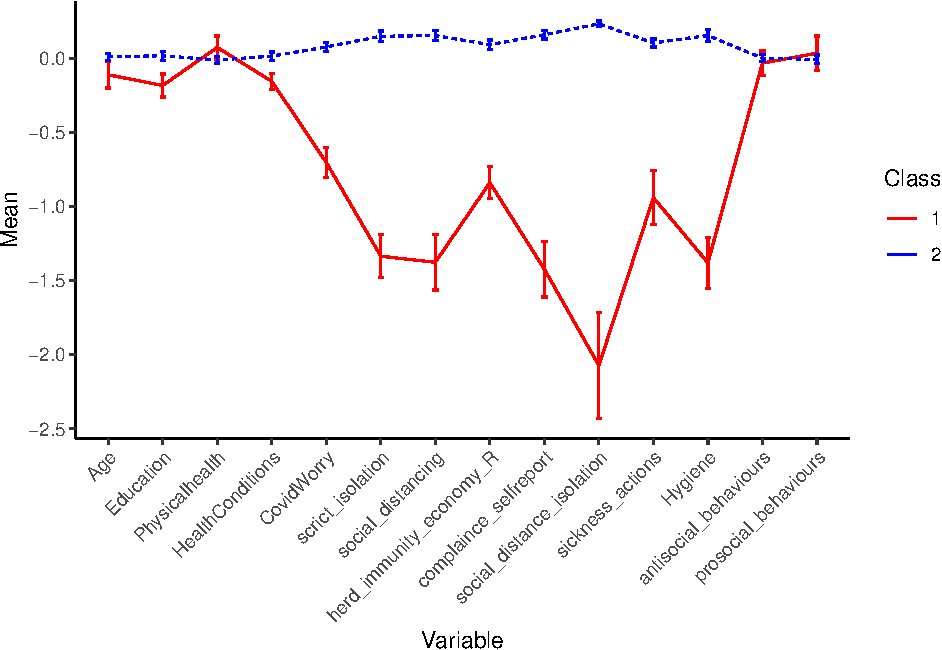
\includegraphics{lpa_analyses_files/figure-latex/unnamed-chunk-5-1.pdf}

\hypertarget{latent-profile-membership}{%
\subsection{Latent profile membership}\label{latent-profile-membership}}

\hypertarget{overall-membership}{%
\subsubsection{Overall membership}\label{overall-membership}}

\begin{table}[H]

\caption{\label{tab:unnamed-chunk-6}Number and percent of participants in each profile}
\centering
\fontsize{6}{8}\selectfont
\begin{tabular}[t]{lrrr}
\toprule
  & 1 & 2 & total\\
\midrule
n & 164 & 1411 & 1575\\
percent & 10 & 90 & 100\\
\bottomrule
\end{tabular}
\end{table}

\hypertarget{country-membership}{%
\subsubsection{Country membership}\label{country-membership}}

\begin{table}[H]

\caption{\label{tab:unnamed-chunk-7}Number of participants from each country in each profile}
\centering
\fontsize{6}{8}\selectfont
\begin{tabular}[t]{lrrr}
\toprule
CountryLive & 1 & 2 & total\\
\midrule
Australia & 72 & 537 & 609\\
Canada & 19 & 284 & 303\\
UK & 21 & 345 & 366\\
US & 52 & 245 & 297\\
\bottomrule
\end{tabular}
\end{table}

\hypertarget{gender-membership}{%
\subsubsection{Gender membership}\label{gender-membership}}

\begin{table}[H]

\caption{\label{tab:unnamed-chunk-8}Number of participants from each gender in each profile}
\centering
\fontsize{6}{8}\selectfont
\begin{tabular}[t]{rrrr}
\toprule
Gender & 1 & 2 & total\\
\midrule
1 & 79 & 473 & 552\\
2 & 85 & 938 & 1023\\
\bottomrule
\end{tabular}
\end{table}

\newpage

\hypertarget{differences-on-out-of-model-variables}{%
\subsubsection{Differences on out of model
variables}\label{differences-on-out-of-model-variables}}

\hypertarget{ordinalcontinuous-variables}{%
\paragraph{Ordinal/Continuous
variables}\label{ordinalcontinuous-variables}}

\begin{table}[H]

\caption{\label{tab:unnamed-chunk-9}Ordinal/continuous variables: Differences between profiles on each variable outside model}
\centering
\fontsize{6}{8}\selectfont
\begin{tabular}[t]{lrrrrlrr}
\toprule
var & mean\_1 & mean\_2 & df & t & p.value & conf.low & conf.high\\
\midrule
CRT\_acc & 45.76 & 48.47 & 462 & -0.58 & 0.564 & -11.90 & 6.49\\
belief\_acc & 53.02 & 56.44 & 460 & -0.81 & 0.416 & -11.68 & 4.84\\
EAT\_acc & 64.45 & 67.95 & 865 & -1.74 & 0.082 & -7.46 & 0.44\\
CRT\_conf & 78.39 & 81.22 & 462 & -1.21 & 0.227 & -7.45 & 1.77\\
belief\_conf & 91.09 & 91.28 & 460 & -0.15 & 0.884 & -2.67 & 2.30\\
\addlinespace
EAT\_conf & 72.91 & 75.40 & 867 & -1.84 & 0.066 & -5.15 & 0.17\\
trait\_conf & 82.22 & 82.97 & 460 & -0.50 & 0.619 & -3.69 & 2.20\\
\textcolor{black}{\textbf{agreeableness}} & \textcolor{black}{\textbf{14.73}} & \textcolor{black}{\textbf{15.73}} & \textcolor{black}{\textbf{1573}} & \textcolor{black}{\textbf{-3.88}} & \textcolor{black}{\textbf{<.001}} & \textcolor{black}{\textbf{-1.50}} & \textcolor{black}{\textbf{-0.49}}\\
conscientious & 13.62 & 13.83 & 1573 & -0.81 & 0.42 & -0.73 & 0.30\\
\textcolor{black}{\textbf{extraversion}} & \textcolor{black}{\textbf{12.14}} & \textcolor{black}{\textbf{11.07}} & \textcolor{black}{\textbf{1573}} & \textcolor{black}{\textbf{3.16}} & \textcolor{black}{\textbf{0.002}} & \textcolor{black}{\textbf{0.40}} & \textcolor{black}{\textbf{1.72}}\\
\addlinespace
\textcolor{black}{\textbf{intellect}} & \textcolor{black}{\textbf{14.67}} & \textcolor{black}{\textbf{15.18}} & \textcolor{black}{\textbf{1573}} & \textcolor{black}{\textbf{-2.02}} & \textcolor{black}{\textbf{0.044}} & \textcolor{black}{\textbf{-1.00}} & \textcolor{black}{\textbf{-0.01}}\\
neuroticism & 11.54 & 11.85 & 1573 & -1.04 & 0.298 & -0.90 & 0.28\\
\textcolor{black}{\textbf{resilience\_adapt}} & \textcolor{black}{\textbf{0.15}} & \textcolor{black}{\textbf{-0.02}} & \textcolor{black}{\textbf{1573}} & \textcolor{black}{\textbf{1.98}} & \textcolor{black}{\textbf{0.048}} & \textcolor{black}{\textbf{0.00}} & \textcolor{black}{\textbf{0.32}}\\
\textcolor{black}{\textbf{cope\_distraction}} & \textcolor{black}{\textbf{5.32}} & \textcolor{black}{\textbf{5.96}} & \textcolor{black}{\textbf{1573}} & \textcolor{black}{\textbf{-5.01}} & \textcolor{black}{\textbf{<.001}} & \textcolor{black}{\textbf{-0.88}} & \textcolor{black}{\textbf{-0.38}}\\
\textcolor{black}{\textbf{cope\_active}} & \textcolor{black}{\textbf{4.73}} & \textcolor{black}{\textbf{5.05}} & \textcolor{black}{\textbf{1573}} & \textcolor{black}{\textbf{-2.47}} & \textcolor{black}{\textbf{0.014}} & \textcolor{black}{\textbf{-0.57}} & \textcolor{black}{\textbf{-0.06}}\\
\addlinespace
\textcolor{black}{\textbf{cope\_denial}} & \textcolor{black}{\textbf{2.82}} & \textcolor{black}{\textbf{2.50}} & \textcolor{black}{\textbf{1573}} & \textcolor{black}{\textbf{3.59}} & \textcolor{black}{\textbf{<.001}} & \textcolor{black}{\textbf{0.14}} & \textcolor{black}{\textbf{0.49}}\\
\textcolor{black}{\textbf{cope\_substance}} & \textcolor{black}{\textbf{3.19}} & \textcolor{black}{\textbf{2.81}} & \textcolor{black}{\textbf{1573}} & \textcolor{black}{\textbf{3.10}} & \textcolor{black}{\textbf{0.002}} & \textcolor{black}{\textbf{0.14}} & \textcolor{black}{\textbf{0.61}}\\
cope\_emotsupp & 4.19 & 4.41 & 1573 & -1.50 & 0.135 & -0.50 & 0.07\\
cope\_instrsupp & 3.80 & 4.04 & 1573 & -1.85 & 0.064 & -0.51 & 0.02\\
\textcolor{black}{\textbf{cope\_disengage}} & \textcolor{black}{\textbf{3.21}} & \textcolor{black}{\textbf{2.91}} & \textcolor{black}{\textbf{1573}} & \textcolor{black}{\textbf{2.87}} & \textcolor{black}{\textbf{0.004}} & \textcolor{black}{\textbf{0.10}} & \textcolor{black}{\textbf{0.52}}\\
\addlinespace
cope\_venting & 3.77 & 3.69 & 1573 & 0.72 & 0.471 & -0.14 & 0.31\\
cope\_reframing & 4.94 & 5.05 & 1573 & -0.83 & 0.407 & -0.39 & 0.16\\
\textcolor{black}{\textbf{cope\_planning}} & \textcolor{black}{\textbf{4.38}} & \textcolor{black}{\textbf{4.89}} & \textcolor{black}{\textbf{1573}} & \textcolor{black}{\textbf{-3.87}} & \textcolor{black}{\textbf{<.001}} & \textcolor{black}{\textbf{-0.77}} & \textcolor{black}{\textbf{-0.25}}\\
PHQ & 39.08 & 38.33 & 405 & 0.40 & 0.689 & -2.95 & 4.45\\
DASS\_stress & 8.38 & 7.25 & 408 & 1.43 & 0.155 & -0.43 & 2.69\\
\addlinespace
DASS\_anxiety & 5.40 & 4.14 & 408 & 1.88 & 0.06 & -0.06 & 2.57\\
DASS\_depression & 6.72 & 6.53 & 408 & 0.24 & 0.811 & -1.38 & 1.77\\
social\_media\_n & 1.96 & 2.00 & 1573 & -0.37 & 0.71 & -0.24 & 0.17\\
\textcolor{black}{\textbf{SourceCheck}} & \textcolor{black}{\textbf{3.17}} & \textcolor{black}{\textbf{3.44}} & \textcolor{black}{\textbf{1573}} & \textcolor{black}{\textbf{-3.02}} & \textcolor{black}{\textbf{0.003}} & \textcolor{black}{\textbf{-0.45}} & \textcolor{black}{\textbf{-0.10}}\\
\textcolor{black}{\textbf{CheckNews}} & \textcolor{black}{\textbf{3.27}} & \textcolor{black}{\textbf{3.72}} & \textcolor{black}{\textbf{1573}} & \textcolor{black}{\textbf{-5.33}} & \textcolor{black}{\textbf{<.001}} & \textcolor{black}{\textbf{-0.61}} & \textcolor{black}{\textbf{-0.28}}\\
\addlinespace
\textcolor{black}{\textbf{official\_sources}} & \textcolor{black}{\textbf{-0.34}} & \textcolor{black}{\textbf{0.04}} & \textcolor{black}{\textbf{1573}} & \textcolor{black}{\textbf{-4.57}} & \textcolor{black}{\textbf{<.001}} & \textcolor{black}{\textbf{-0.54}} & \textcolor{black}{\textbf{-0.21}}\\
casual\_sources & -0.10 & 0.01 & 1573 & -1.29 & 0.198 & -0.27 & 0.06\\
\textcolor{black}{\textbf{official\_trust}} & \textcolor{black}{\textbf{-0.59}} & \textcolor{black}{\textbf{0.07}} & \textcolor{black}{\textbf{1573}} & \textcolor{black}{\textbf{-8.18}} & \textcolor{black}{\textbf{<.001}} & \textcolor{black}{\textbf{-0.82}} & \textcolor{black}{\textbf{-0.50}}\\
\textcolor{black}{\textbf{casual\_trust}} & \textcolor{black}{\textbf{-0.19}} & \textcolor{black}{\textbf{0.02}} & \textcolor{black}{\textbf{1573}} & \textcolor{black}{\textbf{-2.60}} & \textcolor{black}{\textbf{0.01}} & \textcolor{black}{\textbf{-0.38}} & \textcolor{black}{\textbf{-0.05}}\\
\textcolor{black}{\textbf{gov\_trust}} & \textcolor{black}{\textbf{0.18}} & \textcolor{black}{\textbf{-0.02}} & \textcolor{black}{\textbf{1573}} & \textcolor{black}{\textbf{2.47}} & \textcolor{black}{\textbf{0.014}} & \textcolor{black}{\textbf{0.04}} & \textcolor{black}{\textbf{0.36}}\\
\addlinespace
conservatism & 9.88 & 9.69 & 1573 & 0.96 & 0.335 & -0.20 & 0.59\\
\textcolor{black}{\textbf{reactance}} & \textcolor{black}{\textbf{43.54}} & \textcolor{black}{\textbf{39.66}} & \textcolor{black}{\textbf{1573}} & \textcolor{black}{\textbf{5.72}} & \textcolor{black}{\textbf{<.001}} & \textcolor{black}{\textbf{2.55}} & \textcolor{black}{\textbf{5.21}}\\
\textcolor{black}{\textbf{cultural\_tightloose}} & \textcolor{black}{\textbf{22.86}} & \textcolor{black}{\textbf{23.79}} & \textcolor{black}{\textbf{1573}} & \textcolor{black}{\textbf{-3.05}} & \textcolor{black}{\textbf{0.002}} & \textcolor{black}{\textbf{-1.53}} & \textcolor{black}{\textbf{-0.33}}\\
RWA & 8.96 & 9.05 & 1573 & -0.47 & 0.638 & -0.46 & 0.28\\
\textcolor{black}{\textbf{morality}} & \textcolor{black}{\textbf{14.98}} & \textcolor{black}{\textbf{13.75}} & \textcolor{black}{\textbf{409}} & \textcolor{black}{\textbf{2.39}} & \textcolor{black}{\textbf{0.017}} & \textcolor{black}{\textbf{0.22}} & \textcolor{black}{\textbf{2.24}}\\
\addlinespace
\textcolor{black}{\textbf{leave\_going\_to\_work}} & \textcolor{black}{\textbf{2.32}} & \textcolor{black}{\textbf{1.71}} & \textcolor{black}{\textbf{938}} & \textcolor{black}{\textbf{5.30}} & \textcolor{black}{\textbf{<.001}} & \textcolor{black}{\textbf{0.38}} & \textcolor{black}{\textbf{0.83}}\\
leave\_walking\_pet & 1.60 & 1.72 & 938 & -1.00 & 0.32 & -0.36 & 0.12\\
\textcolor{black}{\textbf{leave\_physical\_activity}} & \textcolor{black}{\textbf{2.94}} & \textcolor{black}{\textbf{2.69}} & \textcolor{black}{\textbf{938}} & \textcolor{black}{\textbf{2.12}} & \textcolor{black}{\textbf{0.034}} & \textcolor{black}{\textbf{0.02}} & \textcolor{black}{\textbf{0.48}}\\
\textcolor{black}{\textbf{leave\_get\_food}} & \textcolor{black}{\textbf{2.64}} & \textcolor{black}{\textbf{2.39}} & \textcolor{black}{\textbf{938}} & \textcolor{black}{\textbf{3.37}} & \textcolor{black}{\textbf{0.001}} & \textcolor{black}{\textbf{0.10}} & \textcolor{black}{\textbf{0.39}}\\
leave\_pharmacy & 1.39 & 1.32 & 938 & 1.22 & 0.221 & -0.04 & 0.18\\
\addlinespace
leave\_medical\_treatment & 1.08 & 1.08 & 938 & -0.17 & 0.862 & -0.07 & 0.06\\
\textcolor{black}{\textbf{leave\_care\_dependents}} & \textcolor{black}{\textbf{1.40}} & \textcolor{black}{\textbf{1.22}} & \textcolor{black}{\textbf{938}} & \textcolor{black}{\textbf{2.55}} & \textcolor{black}{\textbf{0.011}} & \textcolor{black}{\textbf{0.04}} & \textcolor{black}{\textbf{0.31}}\\
\textcolor{black}{\textbf{leave\_meet\_friends\_family}} & \textcolor{black}{\textbf{1.87}} & \textcolor{black}{\textbf{1.25}} & \textcolor{black}{\textbf{938}} & \textcolor{black}{\textbf{10.32}} & \textcolor{black}{\textbf{<.001}} & \textcolor{black}{\textbf{0.51}} & \textcolor{black}{\textbf{0.74}}\\
\textcolor{black}{\textbf{leave\_religion}} & \textcolor{black}{\textbf{1.14}} & \textcolor{black}{\textbf{1.02}} & \textcolor{black}{\textbf{935}} & \textcolor{black}{\textbf{4.50}} & \textcolor{black}{\textbf{<.001}} & \textcolor{black}{\textbf{0.07}} & \textcolor{black}{\textbf{0.18}}\\
\textcolor{black}{\textbf{leave\_bored}} & \textcolor{black}{\textbf{2.53}} & \textcolor{black}{\textbf{1.83}} & \textcolor{black}{\textbf{938}} & \textcolor{black}{\textbf{6.36}} & \textcolor{black}{\textbf{<.001}} & \textcolor{black}{\textbf{0.48}} & \textcolor{black}{\textbf{0.91}}\\
\addlinespace
\textcolor{black}{\textbf{leave\_exercise\_freedom}} & \textcolor{black}{\textbf{2.19}} & \textcolor{black}{\textbf{1.34}} & \textcolor{black}{\textbf{938}} & \textcolor{black}{\textbf{9.62}} & \textcolor{black}{\textbf{<.001}} & \textcolor{black}{\textbf{0.67}} & \textcolor{black}{\textbf{1.01}}\\
FinancialSit & 1.74 & 1.72 & 1573 & 0.32 & 0.751 & -0.08 & 0.12\\
worksupportedworkinghome & -0.09 & -0.01 & 426 & -0.44 & 0.662 & -0.45 & 0.29\\
businessokayworkinghome & -0.14 & 0.01 & 91 & -0.48 & 0.63 & -0.77 & 0.47\\
NumberDeaths & 23786.25 & 1834172.34 & 1535 & -0.34 & 0.735 & -12318909.19 & 8698137.01\\
\addlinespace
\textcolor{black}{\textbf{PublicReact}} & \textcolor{black}{\textbf{3.04}} & \textcolor{black}{\textbf{2.51}} & \textcolor{black}{\textbf{1535}} & \textcolor{black}{\textbf{8.01}} & \textcolor{black}{\textbf{<.001}} & \textcolor{black}{\textbf{0.40}} & \textcolor{black}{\textbf{0.66}}\\
CovidLength & 3.57 & 3.72 & 1535 & -1.13 & 0.258 & -0.41 & 0.11\\
HouseholdNumber & 3.06 & 3.11 & 1504 & -0.38 & 0.702 & -0.29 & 0.19\\
\bottomrule
\end{tabular}
\end{table}

\newpage

\begin{center}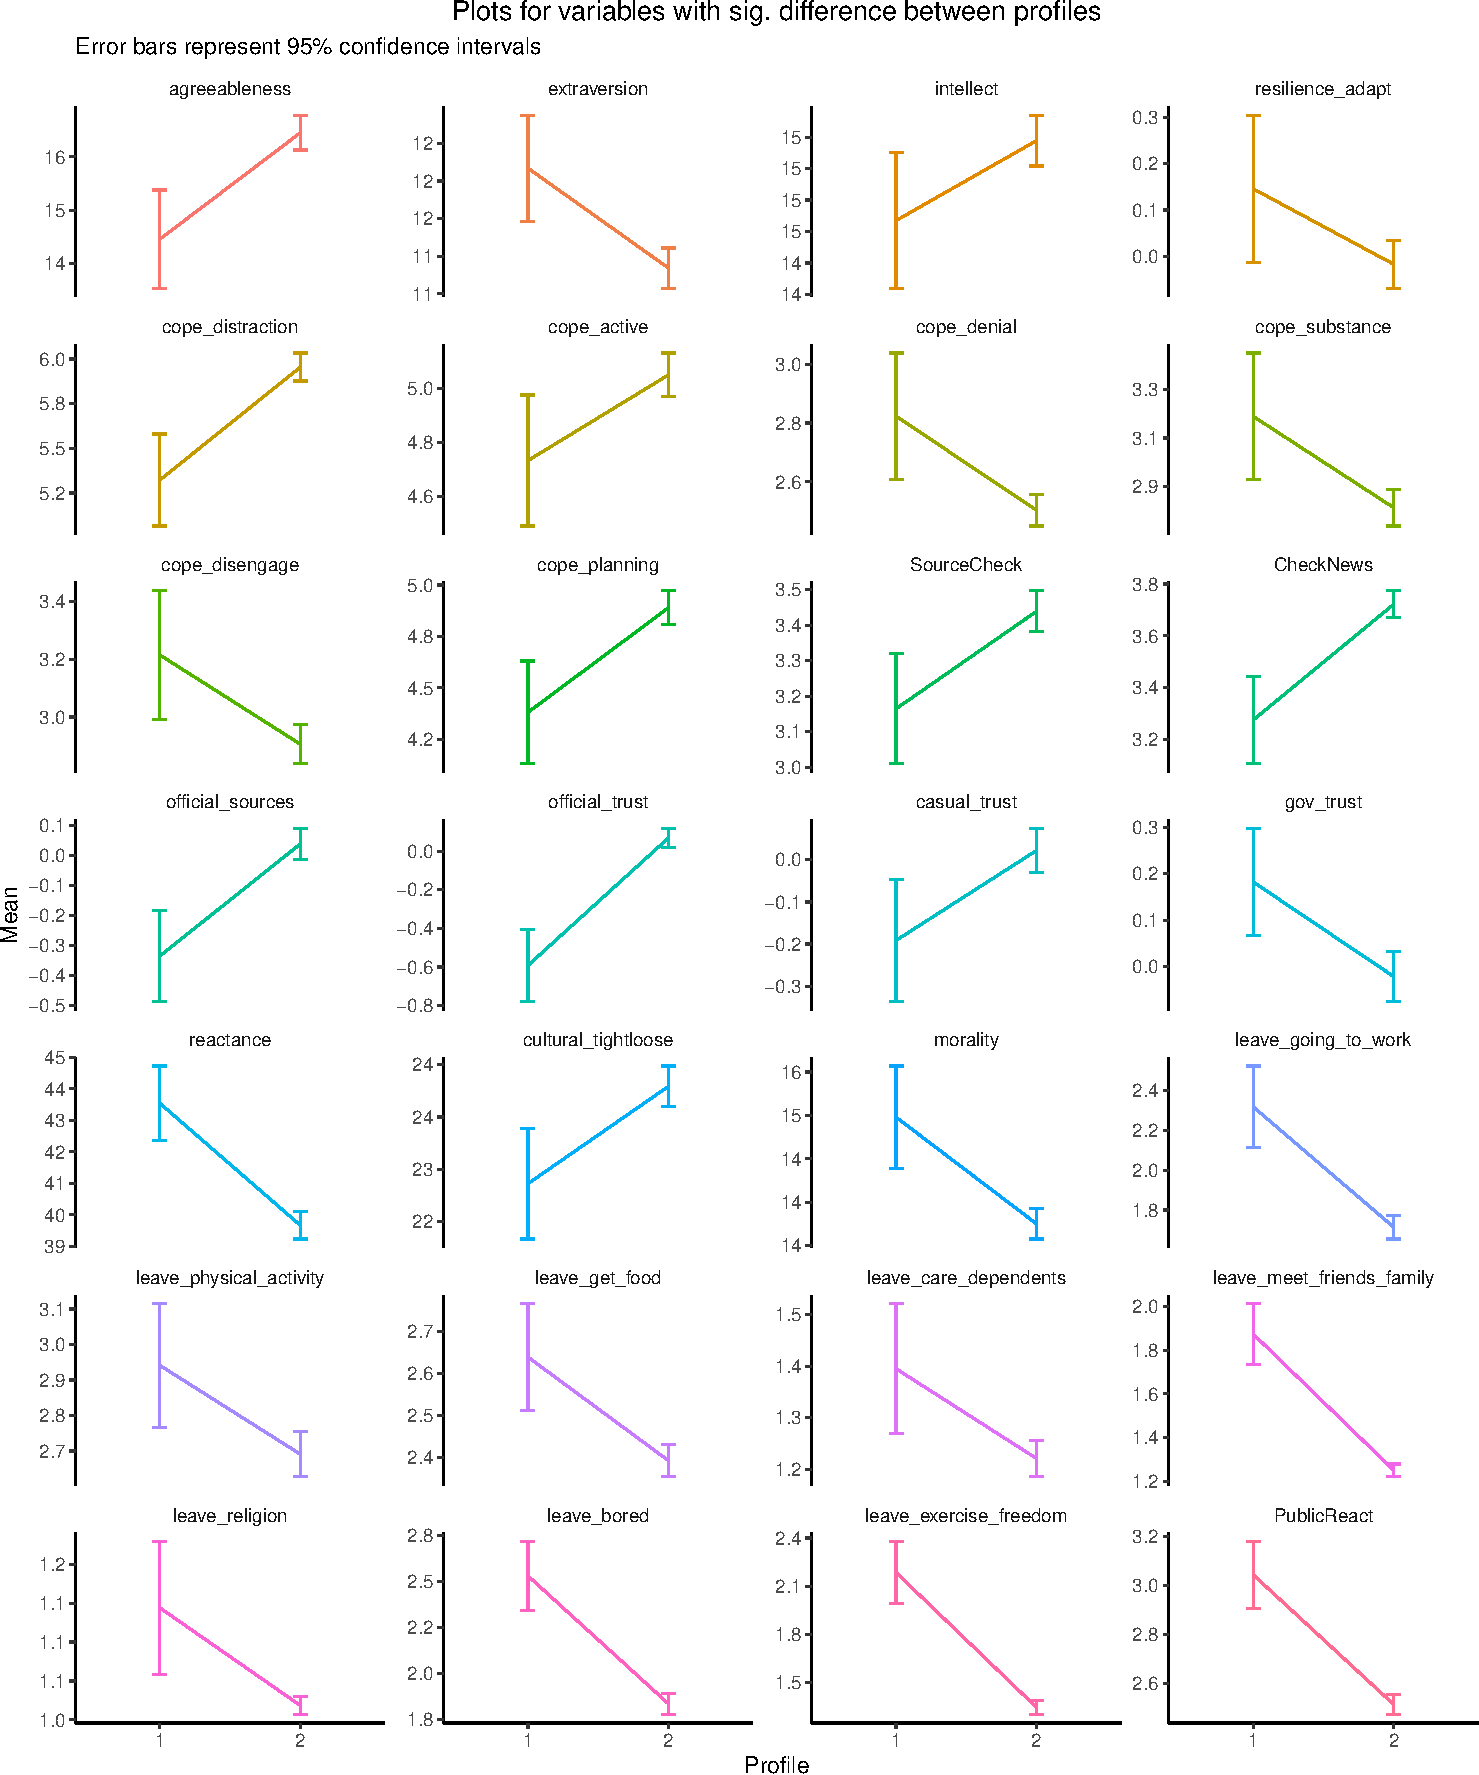
\includegraphics{lpa_analyses_files/figure-latex/unnamed-chunk-10-1} \end{center}

\newpage

\hypertarget{categorical-variables}{%
\paragraph{categorical variables}\label{categorical-variables}}

Chi-square test was used for categorical variables. if an observerd
frequency was less than 5 in a single cell then Fisher's Exact test was
used.

\begin{table}[H]

\caption{\label{tab:unnamed-chunk-11}Categorical variables (Chi-square): Differences between profiles on each variable outside model}
\centering
\fontsize{6}{8}\selectfont
\begin{tabular}[t]{lrrl}
\toprule
var & df & chi\_sq & p.value\\
\midrule
Children & 1 & 0.34 & 0.557\\
\textcolor{black}{\textbf{CountryLive}} & \textcolor{black}{\textbf{3}} & \textcolor{black}{\textbf{31.48}} & \textcolor{black}{\textbf{<.001}}\\
Elderly & 1 & 0.04 & 0.852\\
ElderlyLive & 1 & 0.43 & 0.511\\
\textcolor{black}{\textbf{Gender}} & \textcolor{black}{\textbf{1}} & \textcolor{black}{\textbf{13.21}} & \textcolor{black}{\textbf{<.001}}\\
\addlinespace
Job & 1 & 0.59 & 0.441\\
Layoff & 1 & 0.25 & 0.617\\
\textcolor{black}{\textbf{LeaveHome}} & \textcolor{black}{\textbf{1}} & \textcolor{black}{\textbf{11.91}} & \textcolor{black}{\textbf{0.001}}\\
MaritalStatus & 3 & 4.08 & 0.253\\
\textcolor{black}{\textbf{Workessential}} & \textcolor{black}{\textbf{2}} & \textcolor{black}{\textbf{7.91}} & \textcolor{black}{\textbf{0.019}}\\
\bottomrule
\end{tabular}
\end{table}

\begin{center}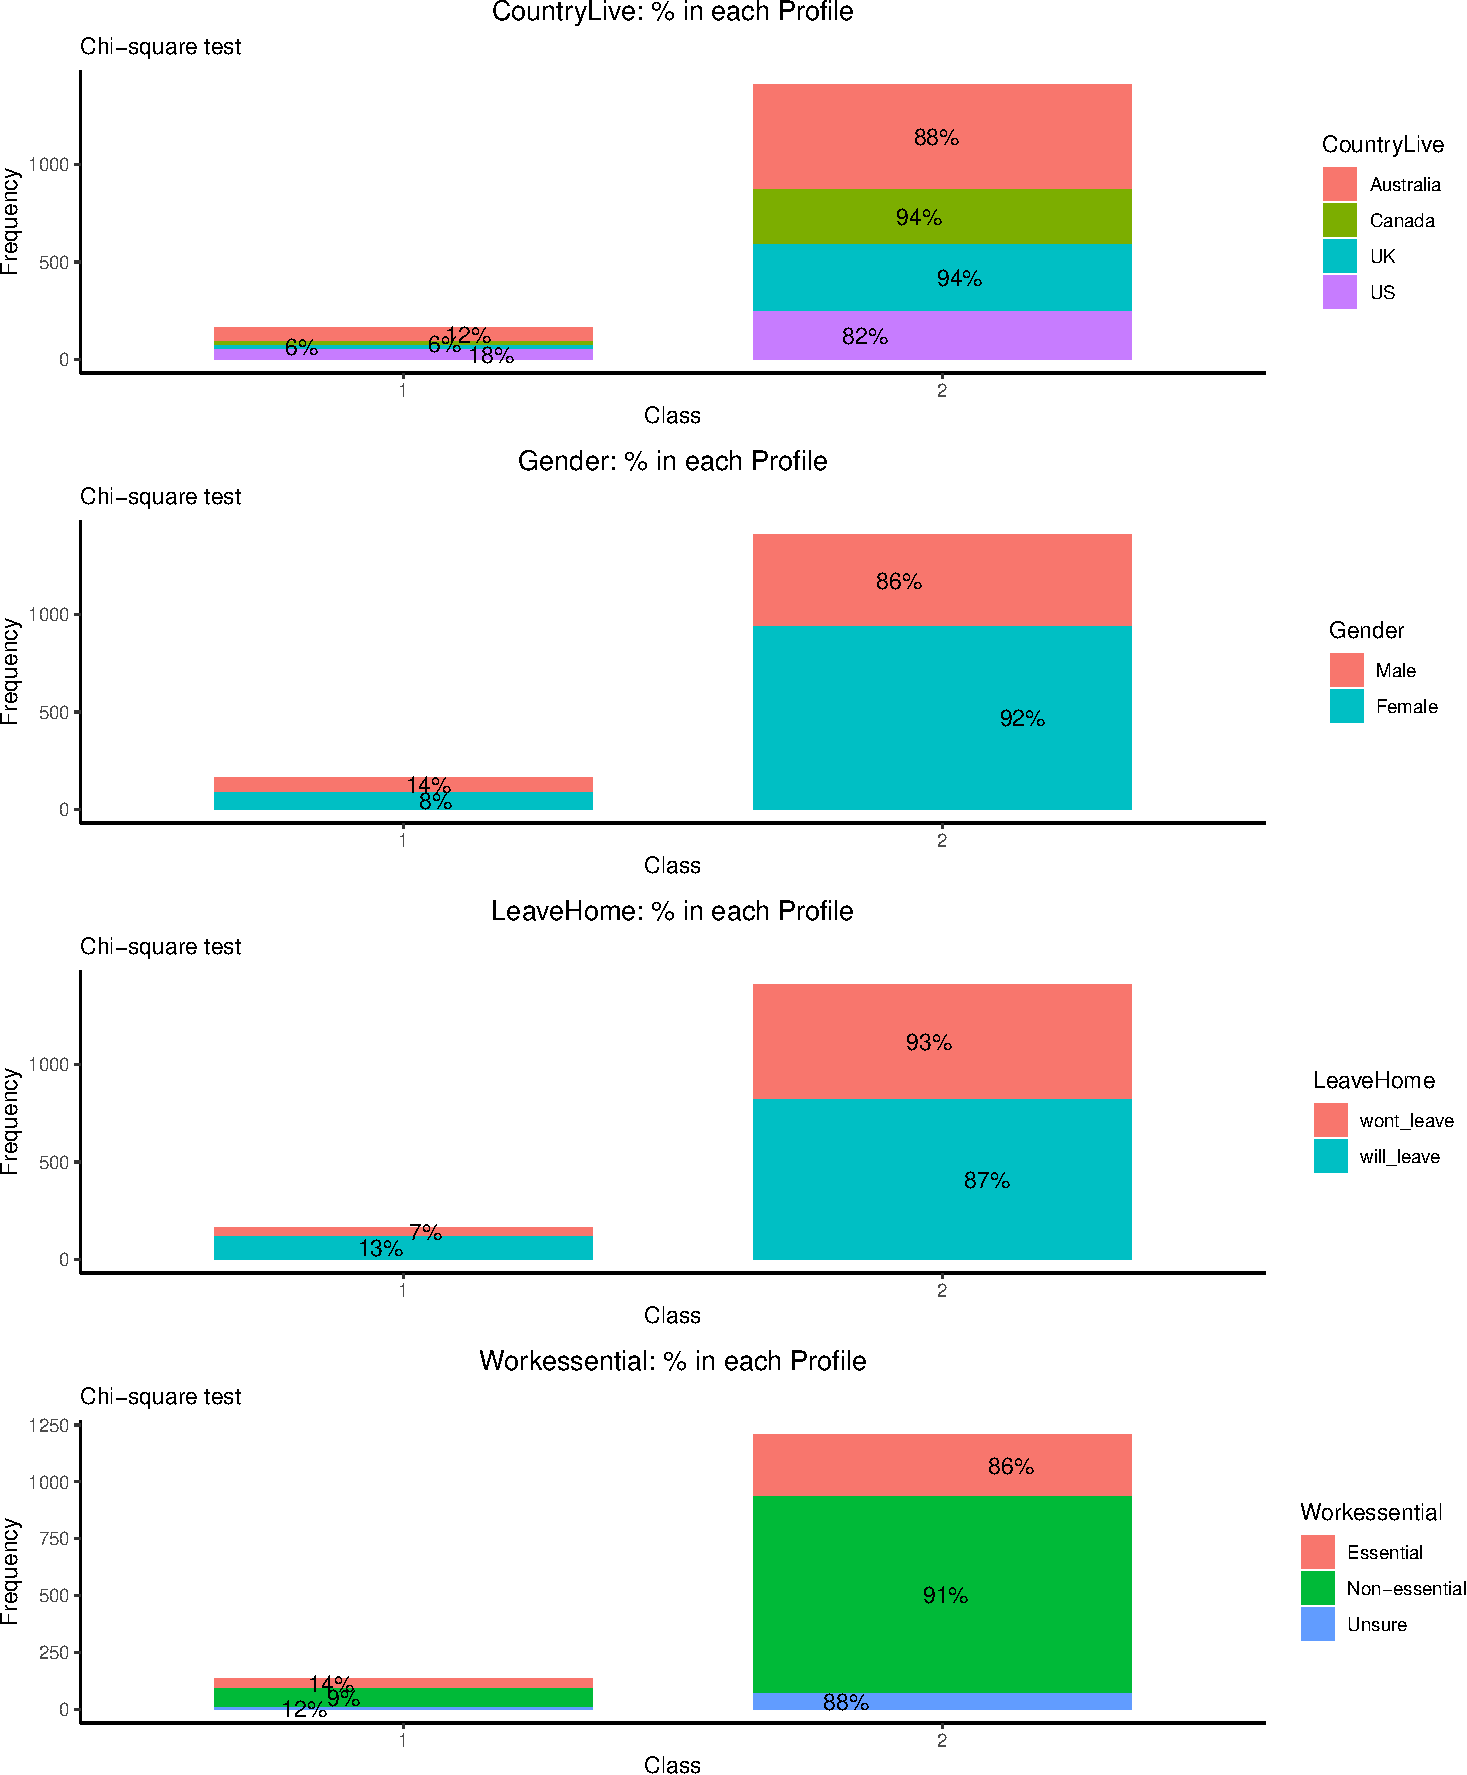
\includegraphics{lpa_analyses_files/figure-latex/unnamed-chunk-11-1} \end{center}

\newpage
\begin{table}[H]

\caption{\label{tab:unnamed-chunk-12}Categorical variables (Fisher's exact): Differences between profiles on each variable outside model}
\centering
\fontsize{6}{8}\selectfont
\begin{tabular}[t]{lr}
\toprule
var & p.value\\
\midrule
LossofJob & 1.00\\
\textcolor{black}{\textbf{Wherework}} & \textcolor{black}{\textbf{0.04}}\\
\bottomrule
\end{tabular}
\end{table}

\begin{center}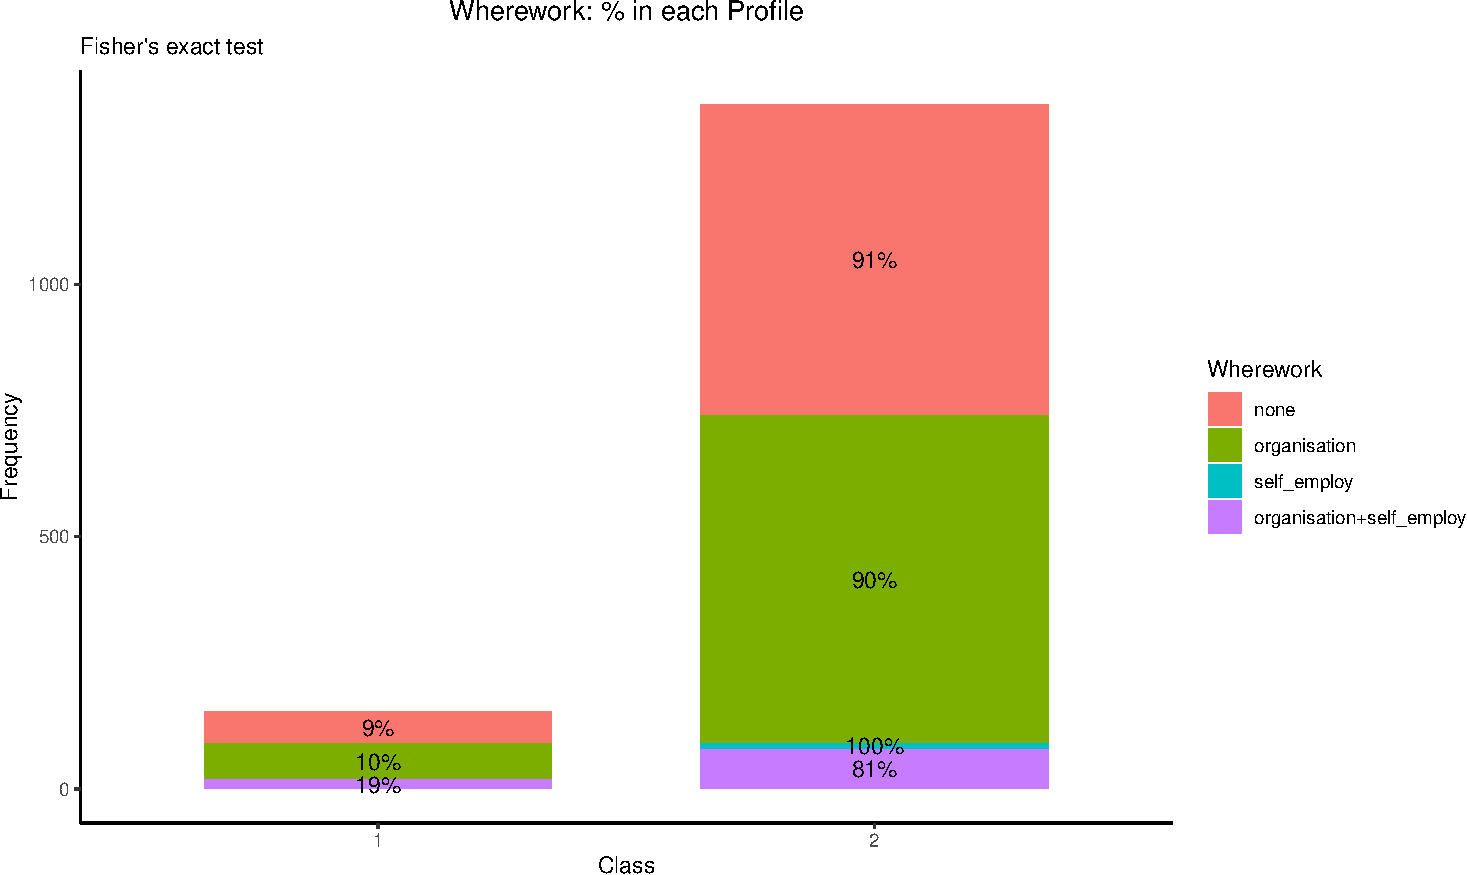
\includegraphics{lpa_analyses_files/figure-latex/unnamed-chunk-12-1} \end{center}

\newpage

\hypertarget{profile-model-1}{%
\section{3 profile model}\label{profile-model-1}}

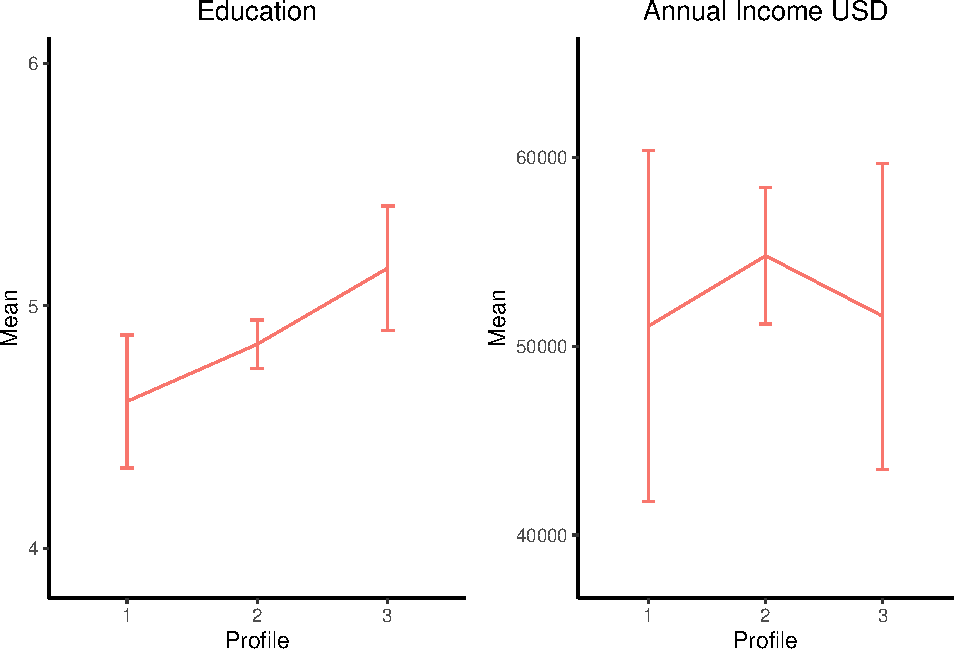
\includegraphics{lpa_analyses_files/figure-latex/unnamed-chunk-13-1.pdf}

\hypertarget{latent-profile-membership-1}{%
\subsection{Latent profile
membership}\label{latent-profile-membership-1}}

\hypertarget{overall-membership-1}{%
\subsubsection{Overall membership}\label{overall-membership-1}}

\begin{table}[H]

\caption{\label{tab:unnamed-chunk-14}Number and percent of participants in each profile}
\centering
\fontsize{6}{8}\selectfont
\begin{tabular}[t]{lrrrr}
\toprule
  & 1 & 2 & 3 & total\\
\midrule
n & 103 & 748 & 724 & 1575\\
percent & 7 & 47 & 46 & 100\\
\bottomrule
\end{tabular}
\end{table}

\hypertarget{country-membership-1}{%
\subsubsection{Country membership}\label{country-membership-1}}

\begin{table}[H]

\caption{\label{tab:unnamed-chunk-15}Number of participants from each country in each profile}
\centering
\fontsize{6}{8}\selectfont
\begin{tabular}[t]{lrrrr}
\toprule
CountryLive & 1 & 2 & 3 & total\\
\midrule
Australia & 46 & 392 & 171 & 609\\
Canada & 12 & 104 & 187 & 303\\
UK & 11 & 157 & 198 & 366\\
US & 34 & 95 & 168 & 297\\
\bottomrule
\end{tabular}
\end{table}

\hypertarget{gender-membership-1}{%
\subsubsection{Gender membership}\label{gender-membership-1}}

\begin{table}[H]

\caption{\label{tab:unnamed-chunk-16}Number of participants from each gender in each profile}
\centering
\fontsize{6}{8}\selectfont
\begin{tabular}[t]{rrrrr}
\toprule
Gender & 1 & 2 & 3 & total\\
\midrule
1 & 47 & 253 & 252 & 552\\
2 & 56 & 495 & 472 & 1023\\
\bottomrule
\end{tabular}
\end{table}

\newpage

\hypertarget{differences-on-out-of-model-variables-1}{%
\subsubsection{Differences on out of model
variables}\label{differences-on-out-of-model-variables-1}}

\hypertarget{ordinalcontinuous-variables-1}{%
\paragraph{Ordinal/Continuous
variables}\label{ordinalcontinuous-variables-1}}

\begin{table}[H]

\caption{\label{tab:unnamed-chunk-17}Ordinal/continuous variables: Differences between profiles on each variable outside model}
\centering
\fontsize{6}{8}\selectfont
\begin{tabular}[t]{lrrrrll}
\toprule
var & SSB & SSW & dfB & dfW & F & p.value\\
\midrule
CRT\_acc & 2984.74 & 518236 & 2 & 461 & 1.33 & 0.266\\
belief\_acc & 3925.30 & 408782 & 2 & 459 & 2.2 & 0.112\\
\textcolor{black}{\textbf{EAT\_acc}} & \textcolor{black}{\textbf{3196.98}} & \textcolor{black}{\textbf{324095}} & \textcolor{black}{\textbf{2}} & \textcolor{black}{\textbf{864}} & \textcolor{black}{\textbf{4.26}} & \textcolor{black}{\textbf{0.014}}\\
CRT\_conf & 806.04 & 130738 & 2 & 461 & 1.42 & 0.243\\
belief\_conf & 18.82 & 37357 & 2 & 459 & 0.12 & 0.891\\
\addlinespace
\textcolor{black}{\textbf{EAT\_conf}} & \textcolor{black}{\textbf{3014.51}} & \textcolor{black}{\textbf{145795}} & \textcolor{black}{\textbf{2}} & \textcolor{black}{\textbf{866}} & \textcolor{black}{\textbf{8.95}} & \textcolor{black}{\textbf{<.001}}\\
trait\_conf & 164.53 & 52136 & 2 & 459 & 0.72 & 0.485\\
\textcolor{black}{\textbf{agreeableness}} & \textcolor{black}{\textbf{122.69}} & \textcolor{black}{\textbf{15275}} & \textcolor{black}{\textbf{2}} & \textcolor{black}{\textbf{1572}} & \textcolor{black}{\textbf{6.31}} & \textcolor{black}{\textbf{0.002}}\\
conscientious & 52.38 & 16026 & 2 & 1572 & 2.57 & 0.077\\
\textcolor{black}{\textbf{extraversion}} & \textcolor{black}{\textbf{170.10}} & \textcolor{black}{\textbf{26110}} & \textcolor{black}{\textbf{2}} & \textcolor{black}{\textbf{1572}} & \textcolor{black}{\textbf{5.12}} & \textcolor{black}{\textbf{0.006}}\\
\addlinespace
intellect & 15.43 & 14751 & 2 & 1572 & 0.82 & 0.44\\
neuroticism & 34.43 & 20723 & 2 & 1572 & 1.31 & 0.271\\
\textcolor{black}{\textbf{resilience\_adapt}} & \textcolor{black}{\textbf{28.38}} & \textcolor{black}{\textbf{1546}} & \textcolor{black}{\textbf{2}} & \textcolor{black}{\textbf{1572}} & \textcolor{black}{\textbf{14.43}} & \textcolor{black}{\textbf{<.001}}\\
\textcolor{black}{\textbf{cope\_distraction}} & \textcolor{black}{\textbf{49.93}} & \textcolor{black}{\textbf{3688}} & \textcolor{black}{\textbf{2}} & \textcolor{black}{\textbf{1572}} & \textcolor{black}{\textbf{10.64}} & \textcolor{black}{\textbf{<.001}}\\
\textcolor{black}{\textbf{cope\_active}} & \textcolor{black}{\textbf{40.60}} & \textcolor{black}{\textbf{3821}} & \textcolor{black}{\textbf{2}} & \textcolor{black}{\textbf{1572}} & \textcolor{black}{\textbf{8.35}} & \textcolor{black}{\textbf{<.001}}\\
\addlinespace
\textcolor{black}{\textbf{cope\_denial}} & \textcolor{black}{\textbf{21.58}} & \textcolor{black}{\textbf{1821}} & \textcolor{black}{\textbf{2}} & \textcolor{black}{\textbf{1572}} & \textcolor{black}{\textbf{9.31}} & \textcolor{black}{\textbf{<.001}}\\
\textcolor{black}{\textbf{cope\_substance}} & \textcolor{black}{\textbf{43.55}} & \textcolor{black}{\textbf{3367}} & \textcolor{black}{\textbf{2}} & \textcolor{black}{\textbf{1572}} & \textcolor{black}{\textbf{10.17}} & \textcolor{black}{\textbf{<.001}}\\
\textcolor{black}{\textbf{cope\_emotsupp}} & \textcolor{black}{\textbf{24.09}} & \textcolor{black}{\textbf{4812}} & \textcolor{black}{\textbf{2}} & \textcolor{black}{\textbf{1572}} & \textcolor{black}{\textbf{3.93}} & \textcolor{black}{\textbf{0.02}}\\
\textcolor{black}{\textbf{cope\_instrsupp}} & \textcolor{black}{\textbf{22.62}} & \textcolor{black}{\textbf{4077}} & \textcolor{black}{\textbf{2}} & \textcolor{black}{\textbf{1572}} & \textcolor{black}{\textbf{4.36}} & \textcolor{black}{\textbf{0.013}}\\
\textcolor{black}{\textbf{cope\_disengage}} & \textcolor{black}{\textbf{12.28}} & \textcolor{black}{\textbf{2697}} & \textcolor{black}{\textbf{2}} & \textcolor{black}{\textbf{1572}} & \textcolor{black}{\textbf{3.58}} & \textcolor{black}{\textbf{0.028}}\\
\addlinespace
cope\_venting & 6.51 & 3057 & 2 & 1572 & 1.68 & 0.188\\
cope\_reframing & 6.09 & 4418 & 2 & 1572 & 1.08 & 0.339\\
\textcolor{black}{\textbf{cope\_planning}} & \textcolor{black}{\textbf{99.77}} & \textcolor{black}{\textbf{3936}} & \textcolor{black}{\textbf{2}} & \textcolor{black}{\textbf{1572}} & \textcolor{black}{\textbf{19.92}} & \textcolor{black}{\textbf{<.001}}\\
PHQ & 104.67 & 62780 & 2 & 404 & 0.34 & 0.714\\
DASS\_stress & 32.69 & 11330 & 2 & 407 & 0.59 & 0.556\\
\addlinespace
DASS\_anxiety & 71.98 & 7956 & 2 & 407 & 1.84 & 0.16\\
DASS\_depression & 6.81 & 11531 & 2 & 407 & 0.12 & 0.887\\
\textcolor{black}{\textbf{social\_media\_n}} & \textcolor{black}{\textbf{20.36}} & \textcolor{black}{\textbf{2487}} & \textcolor{black}{\textbf{2}} & \textcolor{black}{\textbf{1572}} & \textcolor{black}{\textbf{6.44}} & \textcolor{black}{\textbf{0.002}}\\
\textcolor{black}{\textbf{SourceCheck}} & \textcolor{black}{\textbf{41.14}} & \textcolor{black}{\textbf{1886}} & \textcolor{black}{\textbf{2}} & \textcolor{black}{\textbf{1572}} & \textcolor{black}{\textbf{17.14}} & \textcolor{black}{\textbf{<.001}}\\
\textcolor{black}{\textbf{CheckNews}} & \textcolor{black}{\textbf{99.64}} & \textcolor{black}{\textbf{1564}} & \textcolor{black}{\textbf{2}} & \textcolor{black}{\textbf{1572}} & \textcolor{black}{\textbf{50.09}} & \textcolor{black}{\textbf{<.001}}\\
\addlinespace
\textcolor{black}{\textbf{official\_sources}} & \textcolor{black}{\textbf{16.45}} & \textcolor{black}{\textbf{1558}} & \textcolor{black}{\textbf{2}} & \textcolor{black}{\textbf{1572}} & \textcolor{black}{\textbf{8.3}} & \textcolor{black}{\textbf{<.001}}\\
\textcolor{black}{\textbf{casual\_sources}} & \textcolor{black}{\textbf{46.66}} & \textcolor{black}{\textbf{1527}} & \textcolor{black}{\textbf{2}} & \textcolor{black}{\textbf{1572}} & \textcolor{black}{\textbf{24.01}} & \textcolor{black}{\textbf{<.001}}\\
\textcolor{black}{\textbf{official\_trust}} & \textcolor{black}{\textbf{57.16}} & \textcolor{black}{\textbf{1517}} & \textcolor{black}{\textbf{2}} & \textcolor{black}{\textbf{1572}} & \textcolor{black}{\textbf{29.62}} & \textcolor{black}{\textbf{<.001}}\\
\textcolor{black}{\textbf{casual\_trust}} & \textcolor{black}{\textbf{7.96}} & \textcolor{black}{\textbf{1566}} & \textcolor{black}{\textbf{2}} & \textcolor{black}{\textbf{1572}} & \textcolor{black}{\textbf{4}} & \textcolor{black}{\textbf{0.019}}\\
\textcolor{black}{\textbf{gov\_trust}} & \textcolor{black}{\textbf{32.91}} & \textcolor{black}{\textbf{1541}} & \textcolor{black}{\textbf{2}} & \textcolor{black}{\textbf{1572}} & \textcolor{black}{\textbf{16.79}} & \textcolor{black}{\textbf{<.001}}\\
\addlinespace
\textcolor{black}{\textbf{conservatism}} & \textcolor{black}{\textbf{93.09}} & \textcolor{black}{\textbf{9272}} & \textcolor{black}{\textbf{2}} & \textcolor{black}{\textbf{1572}} & \textcolor{black}{\textbf{7.89}} & \textcolor{black}{\textbf{<.001}}\\
\textcolor{black}{\textbf{reactance}} & \textcolor{black}{\textbf{2343.04}} & \textcolor{black}{\textbf{106168}} & \textcolor{black}{\textbf{2}} & \textcolor{black}{\textbf{1572}} & \textcolor{black}{\textbf{17.35}} & \textcolor{black}{\textbf{<.001}}\\
\textcolor{black}{\textbf{cultural\_tightloose}} & \textcolor{black}{\textbf{183.83}} & \textcolor{black}{\textbf{21373}} & \textcolor{black}{\textbf{2}} & \textcolor{black}{\textbf{1572}} & \textcolor{black}{\textbf{6.76}} & \textcolor{black}{\textbf{0.001}}\\
\textcolor{black}{\textbf{RWA}} & \textcolor{black}{\textbf{76.67}} & \textcolor{black}{\textbf{8275}} & \textcolor{black}{\textbf{2}} & \textcolor{black}{\textbf{1572}} & \textcolor{black}{\textbf{7.28}} & \textcolor{black}{\textbf{0.001}}\\
morality & 59.38 & 4746 & 2 & 408 & 2.55 & 0.079\\
\addlinespace
\textcolor{black}{\textbf{leave\_going\_to\_work}} & \textcolor{black}{\textbf{33.66}} & \textcolor{black}{\textbf{1278}} & \textcolor{black}{\textbf{2}} & \textcolor{black}{\textbf{937}} & \textcolor{black}{\textbf{12.34}} & \textcolor{black}{\textbf{<.001}}\\
leave\_walking\_pet & 1.13 & 1463 & 2 & 937 & 0.36 & 0.696\\
\textcolor{black}{\textbf{leave\_physical\_activity}} & \textcolor{black}{\textbf{22.00}} & \textcolor{black}{\textbf{1343}} & \textcolor{black}{\textbf{2}} & \textcolor{black}{\textbf{937}} & \textcolor{black}{\textbf{7.68}} & \textcolor{black}{\textbf{<.001}}\\
\textcolor{black}{\textbf{leave\_get\_food}} & \textcolor{black}{\textbf{5.53}} & \textcolor{black}{\textbf{522}} & \textcolor{black}{\textbf{2}} & \textcolor{black}{\textbf{937}} & \textcolor{black}{\textbf{4.96}} & \textcolor{black}{\textbf{0.007}}\\
leave\_pharmacy & 0.58 & 318 & 2 & 937 & 0.86 & 0.423\\
\addlinespace
leave\_medical\_treatment & 0.10 & 116 & 2 & 937 & 0.4 & 0.671\\
\textcolor{black}{\textbf{leave\_care\_dependents}} & \textcolor{black}{\textbf{6.12}} & \textcolor{black}{\textbf{453}} & \textcolor{black}{\textbf{2}} & \textcolor{black}{\textbf{937}} & \textcolor{black}{\textbf{6.33}} & \textcolor{black}{\textbf{0.002}}\\
\textcolor{black}{\textbf{leave\_meet\_friends\_family}} & \textcolor{black}{\textbf{44.23}} & \textcolor{black}{\textbf{353}} & \textcolor{black}{\textbf{2}} & \textcolor{black}{\textbf{937}} & \textcolor{black}{\textbf{58.67}} & \textcolor{black}{\textbf{<.001}}\\
\textcolor{black}{\textbf{leave\_religion}} & \textcolor{black}{\textbf{2.38}} & \textcolor{black}{\textbf{75}} & \textcolor{black}{\textbf{2}} & \textcolor{black}{\textbf{934}} & \textcolor{black}{\textbf{14.88}} & \textcolor{black}{\textbf{<.001}}\\
\textcolor{black}{\textbf{leave\_bored}} & \textcolor{black}{\textbf{55.29}} & \textcolor{black}{\textbf{1165}} & \textcolor{black}{\textbf{2}} & \textcolor{black}{\textbf{937}} & \textcolor{black}{\textbf{22.24}} & \textcolor{black}{\textbf{<.001}}\\
\addlinespace
\textcolor{black}{\textbf{leave\_exercise\_freedom}} & \textcolor{black}{\textbf{81.51}} & \textcolor{black}{\textbf{737}} & \textcolor{black}{\textbf{2}} & \textcolor{black}{\textbf{937}} & \textcolor{black}{\textbf{51.8}} & \textcolor{black}{\textbf{<.001}}\\
\textcolor{black}{\textbf{FinancialSit}} & \textcolor{black}{\textbf{3.79}} & \textcolor{black}{\textbf{594}} & \textcolor{black}{\textbf{2}} & \textcolor{black}{\textbf{1572}} & \textcolor{black}{\textbf{5.02}} & \textcolor{black}{\textbf{0.007}}\\
\textcolor{black}{\textbf{worksupportedworkinghome}} & \textcolor{black}{\textbf{7.08}} & \textcolor{black}{\textbf{423}} & \textcolor{black}{\textbf{2}} & \textcolor{black}{\textbf{425}} & \textcolor{black}{\textbf{3.56}} & \textcolor{black}{\textbf{0.029}}\\
businessokayworkinghome & 2.68 & 90 & 2 & 90 & 1.34 & 0.267\\
NumberDeaths & 4845789461934100.00 & 6240984855027569664 & 2 & 1534 & 0.6 & 0.551\\
\addlinespace
\textcolor{black}{\textbf{PublicReact}} & \textcolor{black}{\textbf{48.18}} & \textcolor{black}{\textbf{945}} & \textcolor{black}{\textbf{2}} & \textcolor{black}{\textbf{1534}} & \textcolor{black}{\textbf{39.11}} & \textcolor{black}{\textbf{<.001}}\\
\textcolor{black}{\textbf{CovidLength}} & \textcolor{black}{\textbf{49.31}} & \textcolor{black}{\textbf{3795}} & \textcolor{black}{\textbf{2}} & \textcolor{black}{\textbf{1534}} & \textcolor{black}{\textbf{9.97}} & \textcolor{black}{\textbf{<.001}}\\
\textcolor{black}{\textbf{HouseholdNumber}} & \textcolor{black}{\textbf{135.91}} & \textcolor{black}{\textbf{2981}} & \textcolor{black}{\textbf{2}} & \textcolor{black}{\textbf{1503}} & \textcolor{black}{\textbf{34.27}} & \textcolor{black}{\textbf{<.001}}\\
\bottomrule
\end{tabular}
\end{table}

\newpage

\begin{center}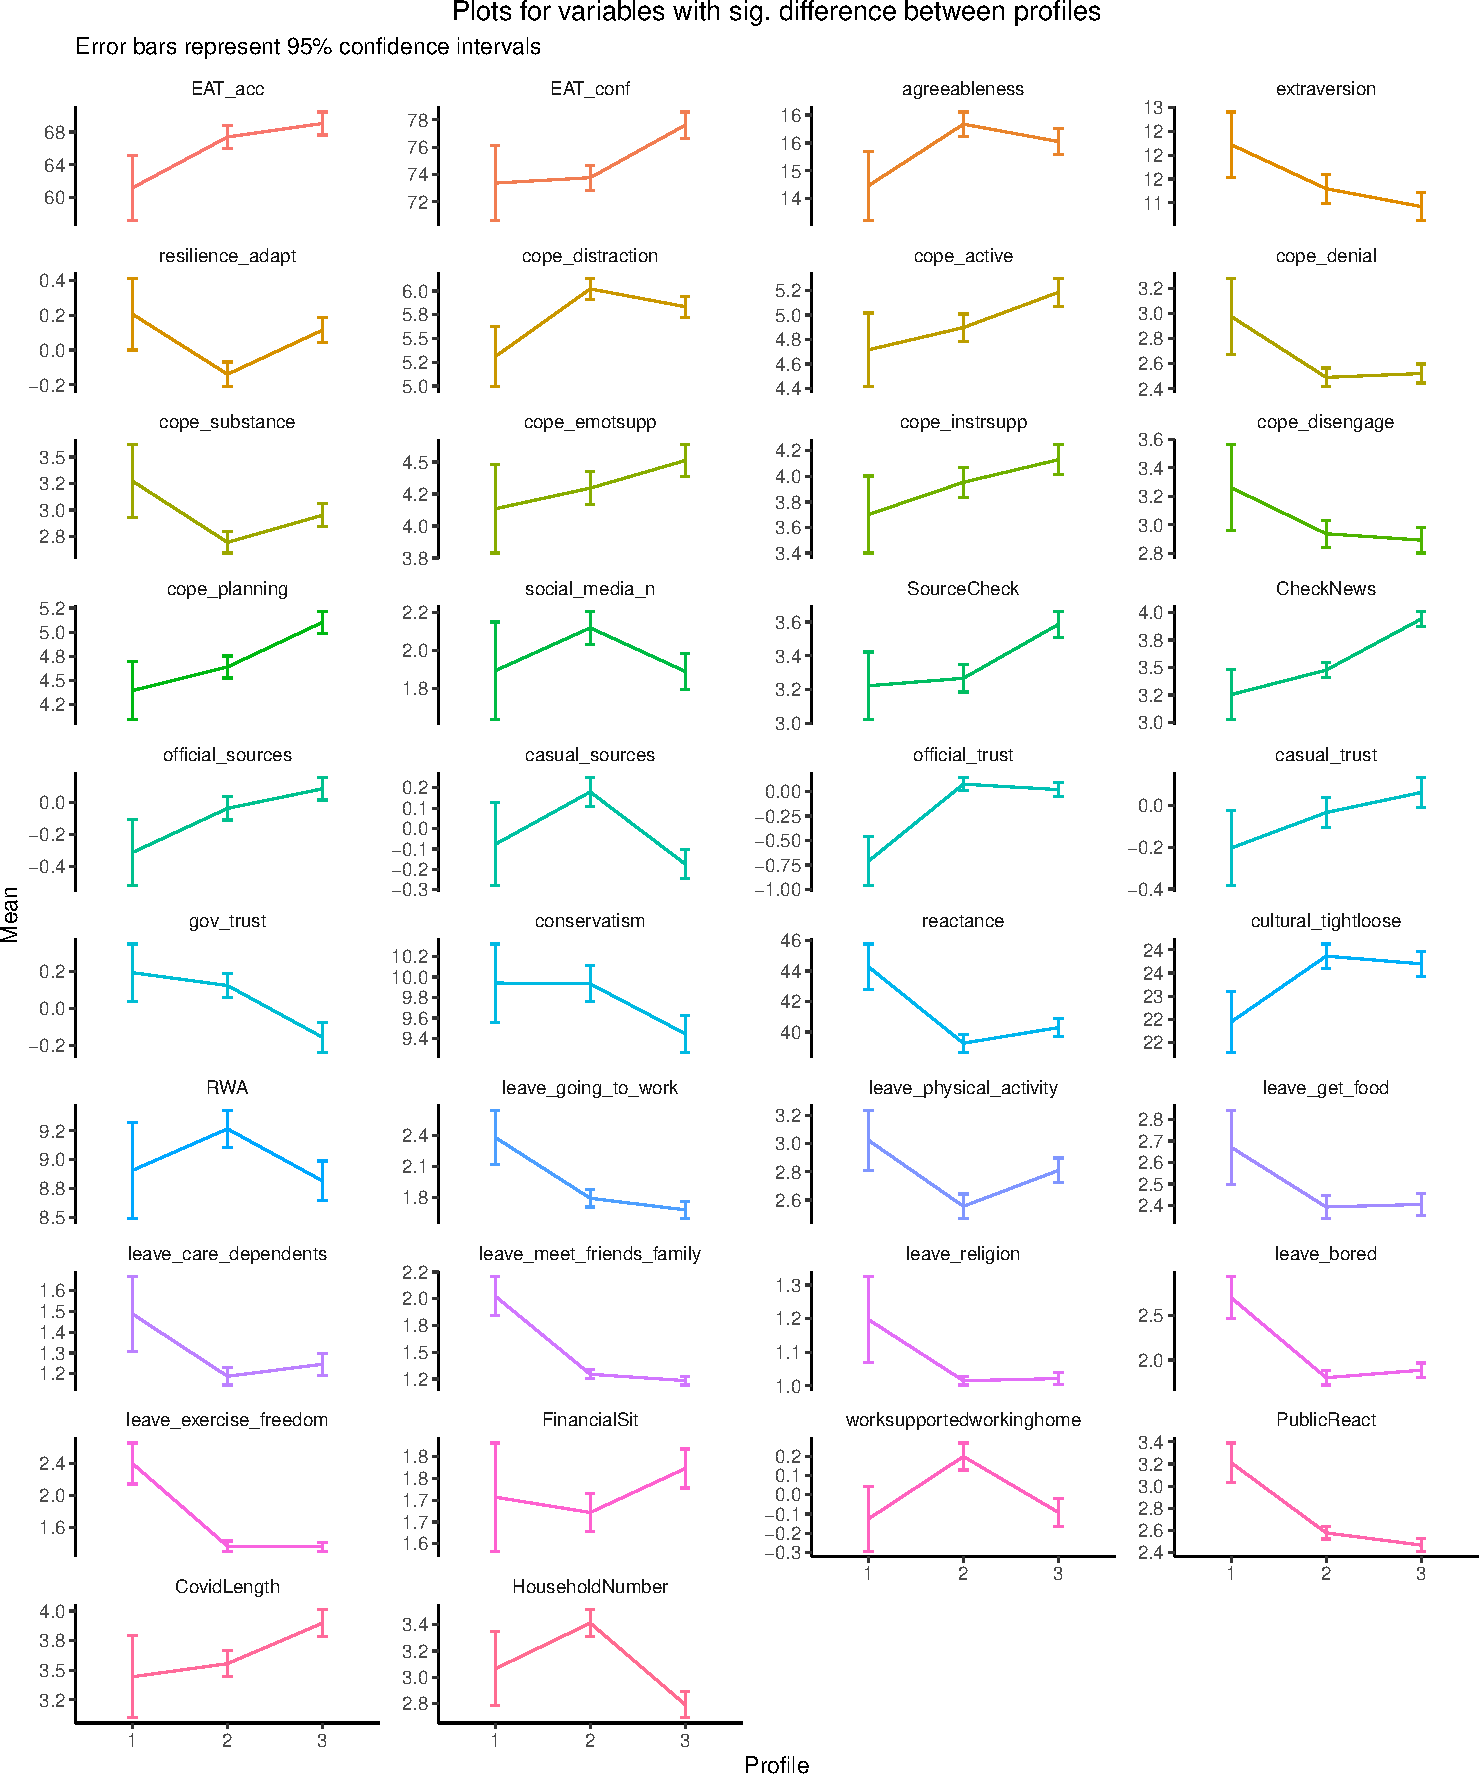
\includegraphics{lpa_analyses_files/figure-latex/unnamed-chunk-18-1} \end{center}

\newpage

\hypertarget{categorical-variables-1}{%
\paragraph{categorical variables}\label{categorical-variables-1}}

\begin{table}[H]

\caption{\label{tab:unnamed-chunk-19}Categorical variables (Chi-square): Differences between profiles on each variable outside model}
\centering
\fontsize{6}{8}\selectfont
\begin{tabular}[t]{lrrl}
\toprule
var & df & chi\_sq & p.value\\
\midrule
\textcolor{black}{\textbf{Children}} & \textcolor{black}{\textbf{2}} & \textcolor{black}{\textbf{27.26}} & \textcolor{black}{\textbf{<.001}}\\
\textcolor{black}{\textbf{CountryLive}} & \textcolor{black}{\textbf{6}} & \textcolor{black}{\textbf{157.48}} & \textcolor{black}{\textbf{<.001}}\\
Elderly & 2 & 0.24 & 0.885\\
ElderlyLive & 2 & 0.69 & 0.71\\
Gender & 2 & 5.58 & 0.061\\
\addlinespace
Job & 2 & 1.85 & 0.397\\
Layoff & 2 & 2.44 & 0.295\\
\textcolor{black}{\textbf{LeaveHome}} & \textcolor{black}{\textbf{2}} & \textcolor{black}{\textbf{37.55}} & \textcolor{black}{\textbf{<.001}}\\
\textcolor{black}{\textbf{MaritalStatus}} & \textcolor{black}{\textbf{6}} & \textcolor{black}{\textbf{117.78}} & \textcolor{black}{\textbf{<.001}}\\
\textcolor{black}{\textbf{Workessential}} & \textcolor{black}{\textbf{4}} & \textcolor{black}{\textbf{12.84}} & \textcolor{black}{\textbf{0.012}}\\
\bottomrule
\end{tabular}
\end{table}

\begin{center}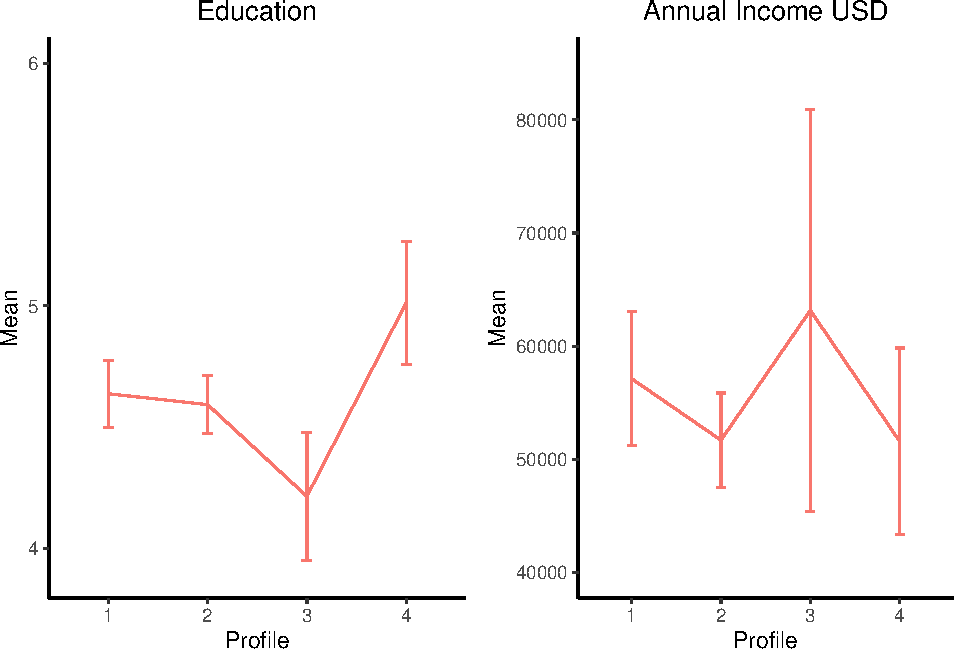
\includegraphics{lpa_analyses_files/figure-latex/unnamed-chunk-19-1} \end{center}

\newpage
\begin{table}[H]

\caption{\label{tab:unnamed-chunk-20}Categorical variables (Fisher's exact): Differences between profiles on each variable outside model}
\centering
\fontsize{6}{8}\selectfont
\begin{tabular}[t]{ll}
\toprule
var & p.value\\
\midrule
LossofJob & 0.764\\
\textcolor{black}{\textbf{Wherework}} & \textcolor{black}{\textbf{<.001}}\\
\bottomrule
\end{tabular}
\end{table}

\begin{center}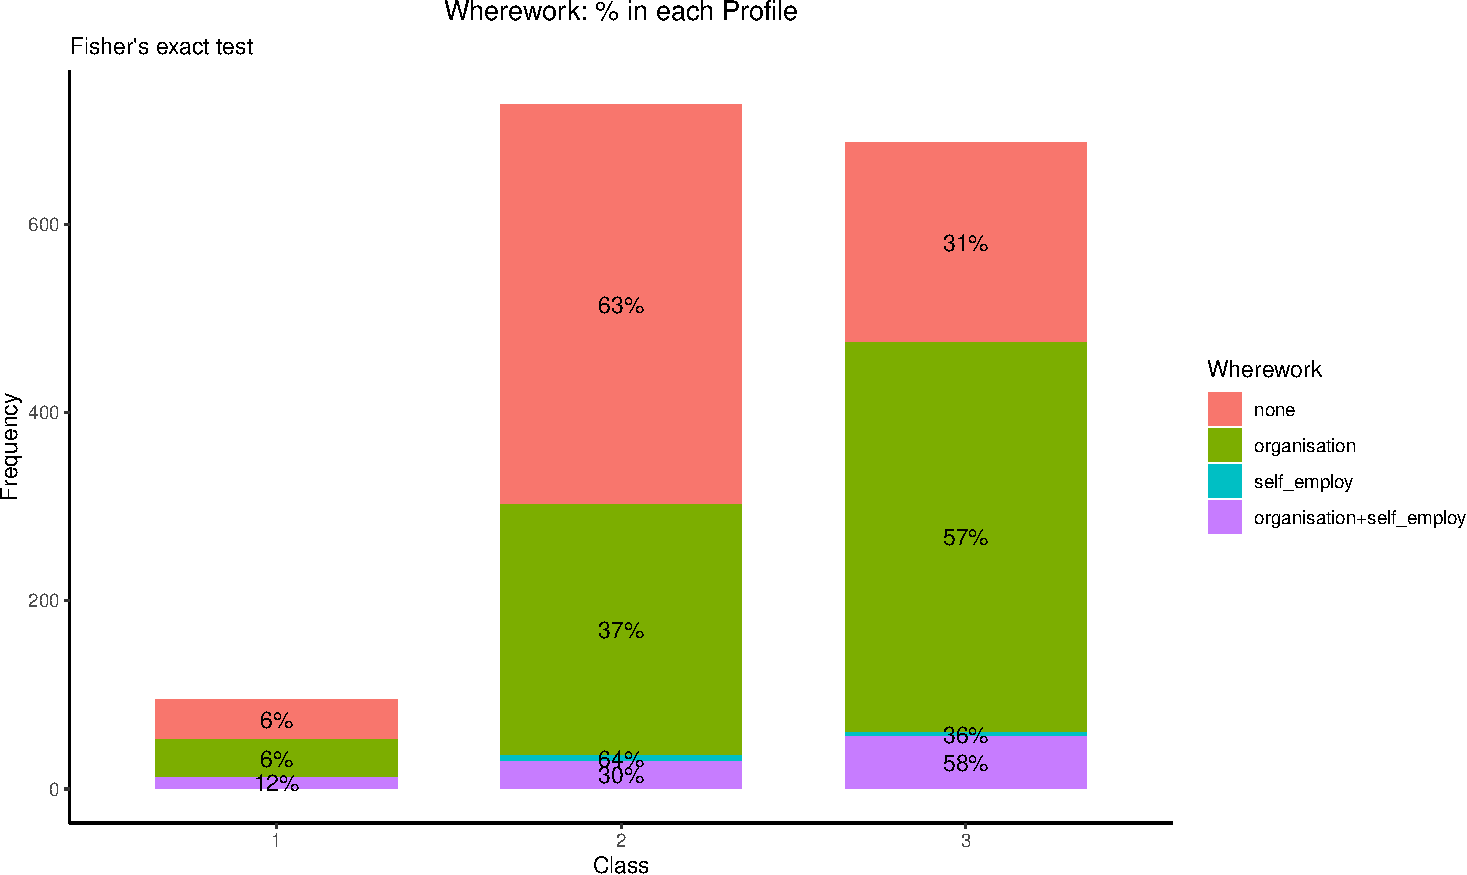
\includegraphics{lpa_analyses_files/figure-latex/unnamed-chunk-20-1} \end{center}

\newpage

\hypertarget{profile-model-2}{%
\section{4 profile model}\label{profile-model-2}}

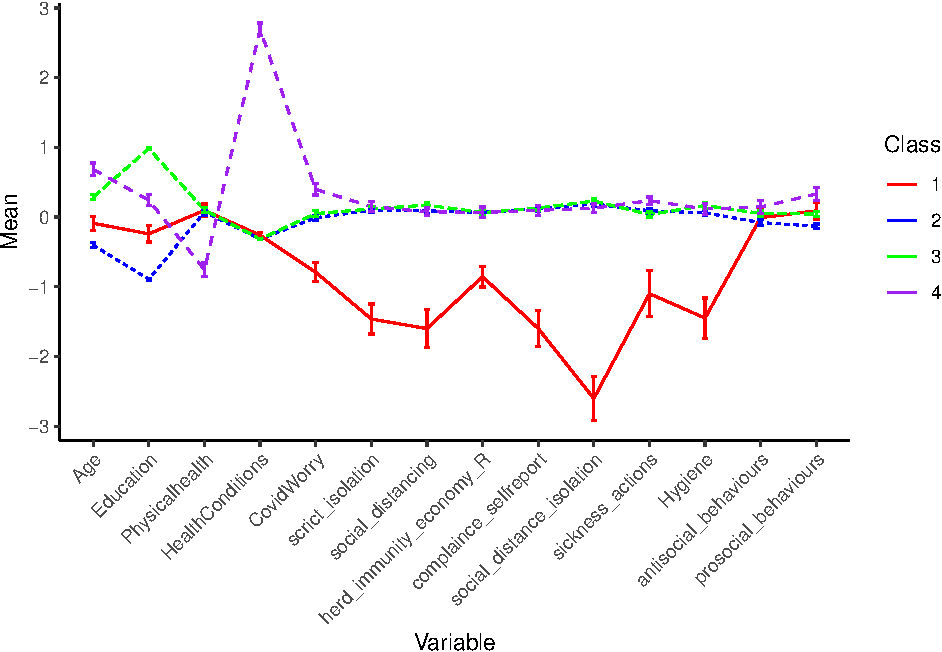
\includegraphics{lpa_analyses_files/figure-latex/unnamed-chunk-21-1.pdf}

\hypertarget{latent-profile-membership-2}{%
\subsection{Latent profile
membership}\label{latent-profile-membership-2}}

\hypertarget{overall-membership-2}{%
\subsubsection{Overall membership}\label{overall-membership-2}}

\begin{table}[H]

\caption{\label{tab:unnamed-chunk-22}Number and percent of participants in each profile}
\centering
\fontsize{6}{8}\selectfont
\begin{tabular}[t]{lrrrrr}
\toprule
  & 1 & 2 & 3 & 4 & total\\
\midrule
n & 112 & 677 & 623 & 163 & 1575\\
percent & 7 & 43 & 40 & 10 & 100\\
\bottomrule
\end{tabular}
\end{table}

\hypertarget{country-membership-2}{%
\subsubsection{Country membership}\label{country-membership-2}}

\begin{table}[H]

\caption{\label{tab:unnamed-chunk-23}Number of participants from each country in each profile}
\centering
\fontsize{6}{8}\selectfont
\begin{tabular}[t]{lrrrrr}
\toprule
CountryLive & 1 & 2 & 3 & 4 & total\\
\midrule
Australia & 50 & 363 & 149 & 47 & 609\\
Canada & 12 & 92 & 161 & 38 & 303\\
UK & 14 & 140 & 175 & 37 & 366\\
US & 36 & 82 & 138 & 41 & 297\\
\bottomrule
\end{tabular}
\end{table}

\hypertarget{gender-membership-2}{%
\subsubsection{Gender membership}\label{gender-membership-2}}

\begin{table}[H]

\caption{\label{tab:unnamed-chunk-24}Number of participants from each gender in each profile}
\centering
\fontsize{6}{8}\selectfont
\begin{tabular}[t]{rrrrrr}
\toprule
Gender & 1 & 2 & 3 & 4 & total\\
\midrule
1 & 53 & 231 & 221 & 47 & 552\\
2 & 59 & 446 & 402 & 116 & 1023\\
\bottomrule
\end{tabular}
\end{table}

\newpage

\hypertarget{differences-on-out-of-model-variables-2}{%
\subsubsection{Differences on out of model
variables}\label{differences-on-out-of-model-variables-2}}

\hypertarget{ordinalcontinuous-variables-2}{%
\paragraph{Ordinal/Continuous
variables}\label{ordinalcontinuous-variables-2}}

\begin{table}[H]

\caption{\label{tab:unnamed-chunk-25}Ordinal/continuous variables: Differences between profiles on each variable outside model}
\centering
\fontsize{6}{8}\selectfont
\begin{tabular}[t]{lrrrrll}
\toprule
var & SSB & SSW & dfB & dfW & F & p.value\\
\midrule
CRT\_acc & 5276.7 & 515944 & 3 & 460 & 1.57 & 0.196\\
belief\_acc & 4688.4 & 408019 & 3 & 458 & 1.75 & 0.155\\
EAT\_acc & 2517.8 & 324774 & 3 & 863 & 2.23 & 0.083\\
CRT\_conf & 1497.0 & 130047 & 3 & 460 & 1.76 & 0.153\\
belief\_conf & 8.3 & 37368 & 3 & 458 & 0.03 & 0.992\\
\addlinespace
\textcolor{black}{\textbf{EAT\_conf}} & \textcolor{black}{\textbf{3367.6}} & \textcolor{black}{\textbf{145442}} & \textcolor{black}{\textbf{3}} & \textcolor{black}{\textbf{865}} & \textcolor{black}{\textbf{6.68}} & \textcolor{black}{\textbf{<.001}}\\
trait\_conf & 173.7 & 52127 & 3 & 458 & 0.51 & 0.676\\
\textcolor{black}{\textbf{agreeableness}} & \textcolor{black}{\textbf{137.3}} & \textcolor{black}{\textbf{15261}} & \textcolor{black}{\textbf{3}} & \textcolor{black}{\textbf{1571}} & \textcolor{black}{\textbf{4.71}} & \textcolor{black}{\textbf{0.003}}\\
conscientious & 52.6 & 16026 & 3 & 1571 & 1.72 & 0.161\\
\textcolor{black}{\textbf{extraversion}} & \textcolor{black}{\textbf{228.6}} & \textcolor{black}{\textbf{26052}} & \textcolor{black}{\textbf{3}} & \textcolor{black}{\textbf{1571}} & \textcolor{black}{\textbf{4.6}} & \textcolor{black}{\textbf{0.003}}\\
\addlinespace
intellect & 10.6 & 14756 & 3 & 1571 & 0.38 & 0.77\\
neuroticism & 28.4 & 20729 & 3 & 1571 & 0.72 & 0.542\\
\textcolor{black}{\textbf{resilience\_adapt}} & \textcolor{black}{\textbf{19.4}} & \textcolor{black}{\textbf{1555}} & \textcolor{black}{\textbf{3}} & \textcolor{black}{\textbf{1571}} & \textcolor{black}{\textbf{6.54}} & \textcolor{black}{\textbf{<.001}}\\
\textcolor{black}{\textbf{cope\_distraction}} & \textcolor{black}{\textbf{45.7}} & \textcolor{black}{\textbf{3692}} & \textcolor{black}{\textbf{3}} & \textcolor{black}{\textbf{1571}} & \textcolor{black}{\textbf{6.48}} & \textcolor{black}{\textbf{<.001}}\\
\textcolor{black}{\textbf{cope\_active}} & \textcolor{black}{\textbf{43.3}} & \textcolor{black}{\textbf{3819}} & \textcolor{black}{\textbf{3}} & \textcolor{black}{\textbf{1571}} & \textcolor{black}{\textbf{5.94}} & \textcolor{black}{\textbf{<.001}}\\
\addlinespace
\textcolor{black}{\textbf{cope\_denial}} & \textcolor{black}{\textbf{22.6}} & \textcolor{black}{\textbf{1820}} & \textcolor{black}{\textbf{3}} & \textcolor{black}{\textbf{1571}} & \textcolor{black}{\textbf{6.51}} & \textcolor{black}{\textbf{<.001}}\\
\textcolor{black}{\textbf{cope\_substance}} & \textcolor{black}{\textbf{59.5}} & \textcolor{black}{\textbf{3351}} & \textcolor{black}{\textbf{3}} & \textcolor{black}{\textbf{1571}} & \textcolor{black}{\textbf{9.29}} & \textcolor{black}{\textbf{<.001}}\\
\textcolor{black}{\textbf{cope\_emotsupp}} & \textcolor{black}{\textbf{34.7}} & \textcolor{black}{\textbf{4802}} & \textcolor{black}{\textbf{3}} & \textcolor{black}{\textbf{1571}} & \textcolor{black}{\textbf{3.79}} & \textcolor{black}{\textbf{0.01}}\\
\textcolor{black}{\textbf{cope\_instrsupp}} & \textcolor{black}{\textbf{21.7}} & \textcolor{black}{\textbf{4078}} & \textcolor{black}{\textbf{3}} & \textcolor{black}{\textbf{1571}} & \textcolor{black}{\textbf{2.79}} & \textcolor{black}{\textbf{0.039}}\\
cope\_disengage & 11.3 & 2698 & 3 & 1571 & 2.19 & 0.088\\
\addlinespace
cope\_venting & 11.7 & 3052 & 3 & 1571 & 2.01 & 0.11\\
cope\_reframing & 6.1 & 4418 & 3 & 1571 & 0.73 & 0.536\\
\textcolor{black}{\textbf{cope\_planning}} & \textcolor{black}{\textbf{72.8}} & \textcolor{black}{\textbf{3963}} & \textcolor{black}{\textbf{3}} & \textcolor{black}{\textbf{1571}} & \textcolor{black}{\textbf{9.62}} & \textcolor{black}{\textbf{<.001}}\\
PHQ & 444.1 & 62441 & 3 & 403 & 0.96 & 0.414\\
DASS\_stress & 18.4 & 11345 & 3 & 406 & 0.22 & 0.883\\
\addlinespace
DASS\_anxiety & 54.1 & 7974 & 3 & 406 & 0.92 & 0.432\\
DASS\_depression & 91.7 & 11446 & 3 & 406 & 1.08 & 0.355\\
\textcolor{black}{\textbf{social\_media\_n}} & \textcolor{black}{\textbf{18.5}} & \textcolor{black}{\textbf{2489}} & \textcolor{black}{\textbf{3}} & \textcolor{black}{\textbf{1571}} & \textcolor{black}{\textbf{3.89}} & \textcolor{black}{\textbf{0.009}}\\
\textcolor{black}{\textbf{SourceCheck}} & \textcolor{black}{\textbf{45.3}} & \textcolor{black}{\textbf{1882}} & \textcolor{black}{\textbf{3}} & \textcolor{black}{\textbf{1571}} & \textcolor{black}{\textbf{12.62}} & \textcolor{black}{\textbf{<.001}}\\
\textcolor{black}{\textbf{CheckNews}} & \textcolor{black}{\textbf{105.6}} & \textcolor{black}{\textbf{1558}} & \textcolor{black}{\textbf{3}} & \textcolor{black}{\textbf{1571}} & \textcolor{black}{\textbf{35.49}} & \textcolor{black}{\textbf{<.001}}\\
\addlinespace
\textcolor{black}{\textbf{official\_sources}} & \textcolor{black}{\textbf{18.0}} & \textcolor{black}{\textbf{1556}} & \textcolor{black}{\textbf{3}} & \textcolor{black}{\textbf{1571}} & \textcolor{black}{\textbf{6.06}} & \textcolor{black}{\textbf{<.001}}\\
\textcolor{black}{\textbf{casual\_sources}} & \textcolor{black}{\textbf{47.9}} & \textcolor{black}{\textbf{1526}} & \textcolor{black}{\textbf{3}} & \textcolor{black}{\textbf{1571}} & \textcolor{black}{\textbf{16.43}} & \textcolor{black}{\textbf{<.001}}\\
\textcolor{black}{\textbf{official\_trust}} & \textcolor{black}{\textbf{54.8}} & \textcolor{black}{\textbf{1519}} & \textcolor{black}{\textbf{3}} & \textcolor{black}{\textbf{1571}} & \textcolor{black}{\textbf{18.9}} & \textcolor{black}{\textbf{<.001}}\\
\textcolor{black}{\textbf{casual\_trust}} & \textcolor{black}{\textbf{9.4}} & \textcolor{black}{\textbf{1565}} & \textcolor{black}{\textbf{3}} & \textcolor{black}{\textbf{1571}} & \textcolor{black}{\textbf{3.15}} & \textcolor{black}{\textbf{0.024}}\\
\textcolor{black}{\textbf{gov\_trust}} & \textcolor{black}{\textbf{35.5}} & \textcolor{black}{\textbf{1538}} & \textcolor{black}{\textbf{3}} & \textcolor{black}{\textbf{1571}} & \textcolor{black}{\textbf{12.09}} & \textcolor{black}{\textbf{<.001}}\\
\addlinespace
\textcolor{black}{\textbf{conservatism}} & \textcolor{black}{\textbf{100.5}} & \textcolor{black}{\textbf{9264}} & \textcolor{black}{\textbf{3}} & \textcolor{black}{\textbf{1571}} & \textcolor{black}{\textbf{5.68}} & \textcolor{black}{\textbf{0.001}}\\
\textcolor{black}{\textbf{reactance}} & \textcolor{black}{\textbf{2292.8}} & \textcolor{black}{\textbf{106219}} & \textcolor{black}{\textbf{3}} & \textcolor{black}{\textbf{1571}} & \textcolor{black}{\textbf{11.3}} & \textcolor{black}{\textbf{<.001}}\\
\textcolor{black}{\textbf{cultural\_tightloose}} & \textcolor{black}{\textbf{114.1}} & \textcolor{black}{\textbf{21443}} & \textcolor{black}{\textbf{3}} & \textcolor{black}{\textbf{1571}} & \textcolor{black}{\textbf{2.79}} & \textcolor{black}{\textbf{0.04}}\\
\textcolor{black}{\textbf{RWA}} & \textcolor{black}{\textbf{71.8}} & \textcolor{black}{\textbf{8280}} & \textcolor{black}{\textbf{3}} & \textcolor{black}{\textbf{1571}} & \textcolor{black}{\textbf{4.54}} & \textcolor{black}{\textbf{0.004}}\\
morality & 79.3 & 4726 & 3 & 407 & 2.27 & 0.079\\
\addlinespace
\textcolor{black}{\textbf{leave\_going\_to\_work}} & \textcolor{black}{\textbf{29.0}} & \textcolor{black}{\textbf{1283}} & \textcolor{black}{\textbf{3}} & \textcolor{black}{\textbf{936}} & \textcolor{black}{\textbf{7.05}} & \textcolor{black}{\textbf{<.001}}\\
leave\_walking\_pet & 3.0 & 1461 & 3 & 936 & 0.64 & 0.587\\
\textcolor{black}{\textbf{leave\_physical\_activity}} & \textcolor{black}{\textbf{27.3}} & \textcolor{black}{\textbf{1337}} & \textcolor{black}{\textbf{3}} & \textcolor{black}{\textbf{936}} & \textcolor{black}{\textbf{6.38}} & \textcolor{black}{\textbf{<.001}}\\
\textcolor{black}{\textbf{leave\_get\_food}} & \textcolor{black}{\textbf{5.5}} & \textcolor{black}{\textbf{522}} & \textcolor{black}{\textbf{3}} & \textcolor{black}{\textbf{936}} & \textcolor{black}{\textbf{3.27}} & \textcolor{black}{\textbf{0.021}}\\
\textcolor{black}{\textbf{leave\_pharmacy}} & \textcolor{black}{\textbf{7.2}} & \textcolor{black}{\textbf{311}} & \textcolor{black}{\textbf{3}} & \textcolor{black}{\textbf{936}} & \textcolor{black}{\textbf{7.2}} & \textcolor{black}{\textbf{<.001}}\\
\addlinespace
\textcolor{black}{\textbf{leave\_medical\_treatment}} & \textcolor{black}{\textbf{4.4}} & \textcolor{black}{\textbf{111}} & \textcolor{black}{\textbf{3}} & \textcolor{black}{\textbf{936}} & \textcolor{black}{\textbf{12.27}} & \textcolor{black}{\textbf{<.001}}\\
\textcolor{black}{\textbf{leave\_care\_dependents}} & \textcolor{black}{\textbf{7.1}} & \textcolor{black}{\textbf{452}} & \textcolor{black}{\textbf{3}} & \textcolor{black}{\textbf{936}} & \textcolor{black}{\textbf{4.9}} & \textcolor{black}{\textbf{0.002}}\\
\textcolor{black}{\textbf{leave\_meet\_friends\_family}} & \textcolor{black}{\textbf{41.6}} & \textcolor{black}{\textbf{356}} & \textcolor{black}{\textbf{3}} & \textcolor{black}{\textbf{936}} & \textcolor{black}{\textbf{36.48}} & \textcolor{black}{\textbf{<.001}}\\
\textcolor{black}{\textbf{leave\_religion}} & \textcolor{black}{\textbf{2.7}} & \textcolor{black}{\textbf{74}} & \textcolor{black}{\textbf{3}} & \textcolor{black}{\textbf{933}} & \textcolor{black}{\textbf{11.25}} & \textcolor{black}{\textbf{<.001}}\\
\textcolor{black}{\textbf{leave\_bored}} & \textcolor{black}{\textbf{52.6}} & \textcolor{black}{\textbf{1168}} & \textcolor{black}{\textbf{3}} & \textcolor{black}{\textbf{936}} & \textcolor{black}{\textbf{14.06}} & \textcolor{black}{\textbf{<.001}}\\
\addlinespace
\textcolor{black}{\textbf{leave\_exercise\_freedom}} & \textcolor{black}{\textbf{65.6}} & \textcolor{black}{\textbf{753}} & \textcolor{black}{\textbf{3}} & \textcolor{black}{\textbf{936}} & \textcolor{black}{\textbf{27.19}} & \textcolor{black}{\textbf{<.001}}\\
\textcolor{black}{\textbf{FinancialSit}} & \textcolor{black}{\textbf{5.9}} & \textcolor{black}{\textbf{592}} & \textcolor{black}{\textbf{3}} & \textcolor{black}{\textbf{1571}} & \textcolor{black}{\textbf{5.21}} & \textcolor{black}{\textbf{0.001}}\\
worksupportedworkinghome & 5.5 & 425 & 3 & 424 & 1.83 & 0.141\\
businessokayworkinghome & 2.8 & 90 & 3 & 89 & 0.92 & 0.433\\
NumberDeaths & 6263881643480407.0 & 6239566762846023680 & 3 & 1533 & 0.51 & 0.673\\
\addlinespace
\textcolor{black}{\textbf{PublicReact}} & \textcolor{black}{\textbf{47.8}} & \textcolor{black}{\textbf{945}} & \textcolor{black}{\textbf{3}} & \textcolor{black}{\textbf{1533}} & \textcolor{black}{\textbf{25.84}} & \textcolor{black}{\textbf{<.001}}\\
\textcolor{black}{\textbf{CovidLength}} & \textcolor{black}{\textbf{72.7}} & \textcolor{black}{\textbf{3771}} & \textcolor{black}{\textbf{3}} & \textcolor{black}{\textbf{1533}} & \textcolor{black}{\textbf{9.85}} & \textcolor{black}{\textbf{<.001}}\\
\textcolor{black}{\textbf{HouseholdNumber}} & \textcolor{black}{\textbf{134.5}} & \textcolor{black}{\textbf{2982}} & \textcolor{black}{\textbf{3}} & \textcolor{black}{\textbf{1502}} & \textcolor{black}{\textbf{22.59}} & \textcolor{black}{\textbf{<.001}}\\
\bottomrule
\end{tabular}
\end{table}

\newpage

\begin{center}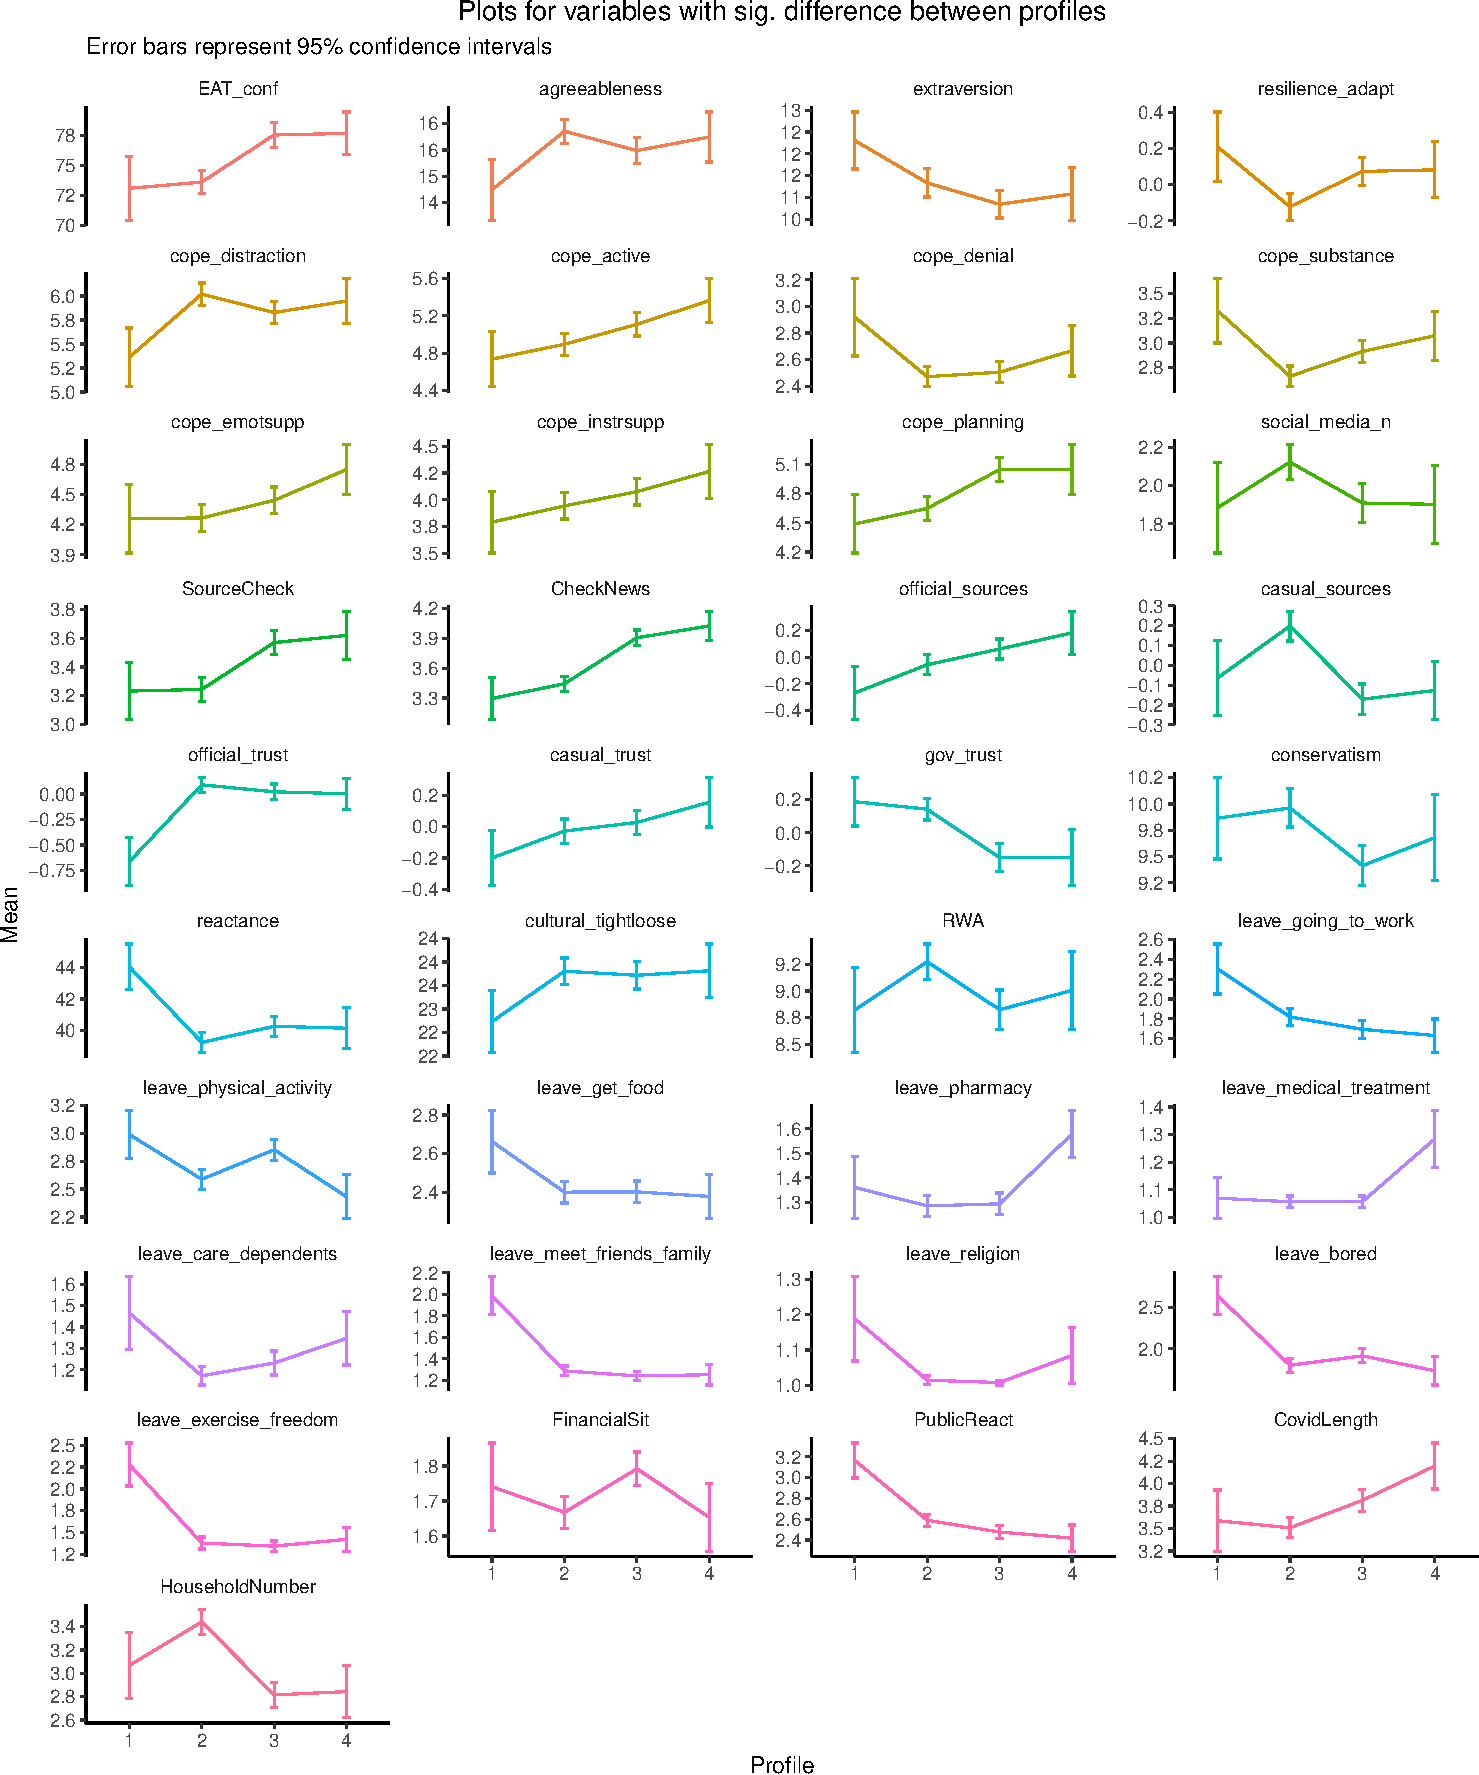
\includegraphics{lpa_analyses_files/figure-latex/unnamed-chunk-26-1} \end{center}

\newpage

\hypertarget{categorical-variables-2}{%
\paragraph{categorical variables}\label{categorical-variables-2}}

\begin{table}[H]

\caption{\label{tab:unnamed-chunk-27}Categorical variables (Chi-square): Differences between profiles on each variable outside model}
\centering
\fontsize{6}{8}\selectfont
\begin{tabular}[t]{lrrl}
\toprule
var & df & chi\_sq & p.value\\
\midrule
\textcolor{black}{\textbf{Children}} & \textcolor{black}{\textbf{3}} & \textcolor{black}{\textbf{22.3}} & \textcolor{black}{\textbf{<.001}}\\
\textcolor{black}{\textbf{CountryLive}} & \textcolor{black}{\textbf{9}} & \textcolor{black}{\textbf{157.9}} & \textcolor{black}{\textbf{<.001}}\\
Elderly & 3 & 1.3 & 0.738\\
ElderlyLive & 3 & 2.0 & 0.574\\
\textcolor{black}{\textbf{Gender}} & \textcolor{black}{\textbf{3}} & \textcolor{black}{\textbf{10.5}} & \textcolor{black}{\textbf{0.015}}\\
\addlinespace
Job & 3 & 2.6 & 0.463\\
Layoff & 3 & 2.8 & 0.432\\
\textcolor{black}{\textbf{LeaveHome}} & \textcolor{black}{\textbf{3}} & \textcolor{black}{\textbf{35.9}} & \textcolor{black}{\textbf{<.001}}\\
\textcolor{black}{\textbf{MaritalStatus}} & \textcolor{black}{\textbf{9}} & \textcolor{black}{\textbf{153.2}} & \textcolor{black}{\textbf{<.001}}\\
\textcolor{black}{\textbf{Workessential}} & \textcolor{black}{\textbf{6}} & \textcolor{black}{\textbf{13.3}} & \textcolor{black}{\textbf{0.039}}\\
\bottomrule
\end{tabular}
\end{table}

\begin{center}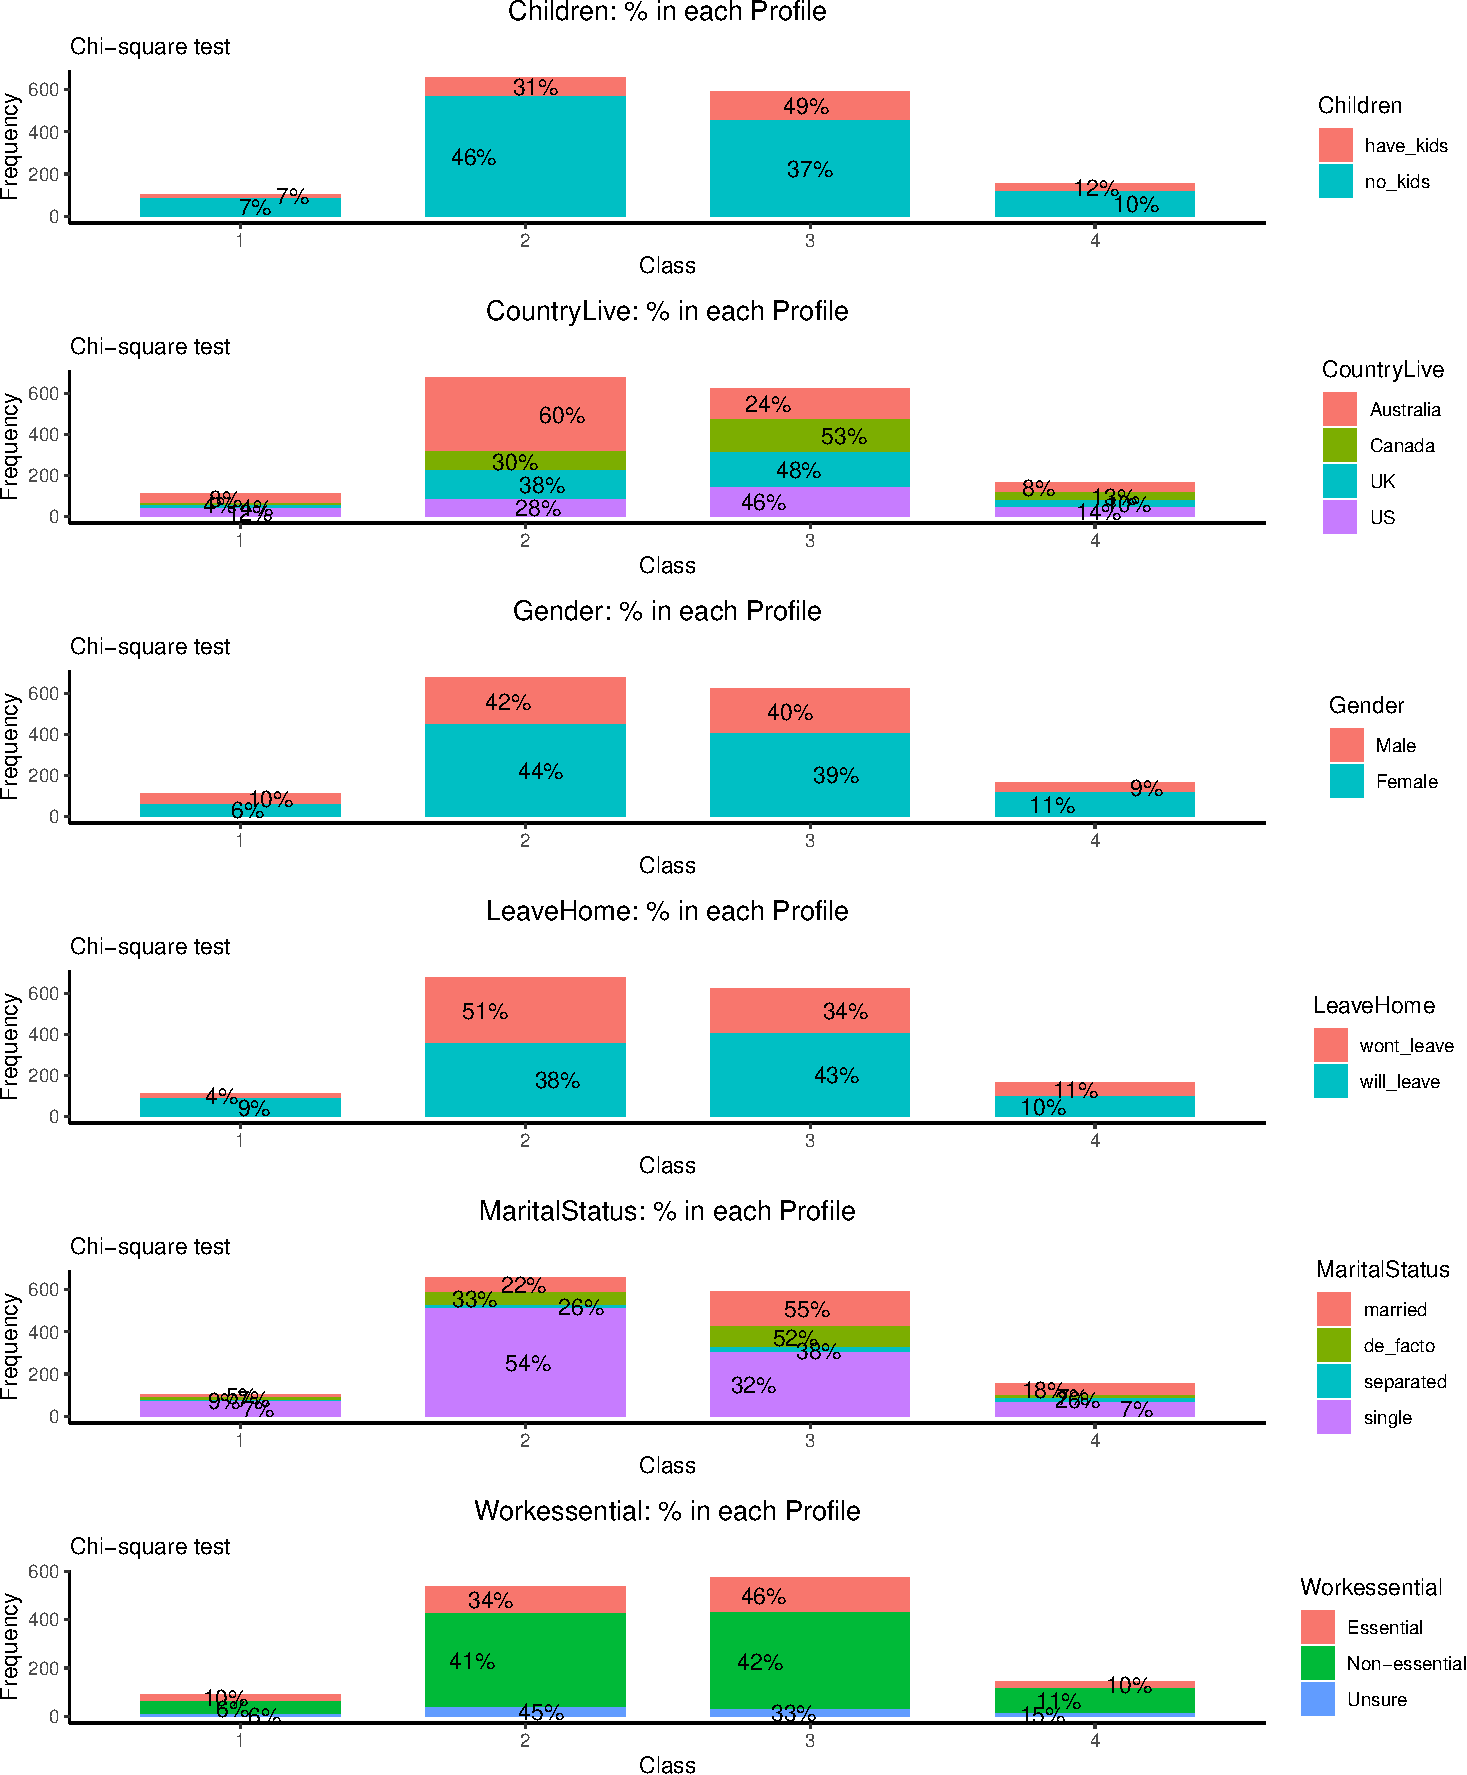
\includegraphics{lpa_analyses_files/figure-latex/unnamed-chunk-27-1} \end{center}

\newpage
\begin{table}[H]

\caption{\label{tab:unnamed-chunk-28}Categorical variables (Fisher's exact): Differences between profiles on each variable outside model}
\centering
\fontsize{6}{8}\selectfont
\begin{tabular}[t]{ll}
\toprule
var & p.value\\
\midrule
LossofJob & 0.945\\
\textcolor{black}{\textbf{Wherework}} & \textcolor{black}{\textbf{<.001}}\\
\bottomrule
\end{tabular}
\end{table}

\begin{center}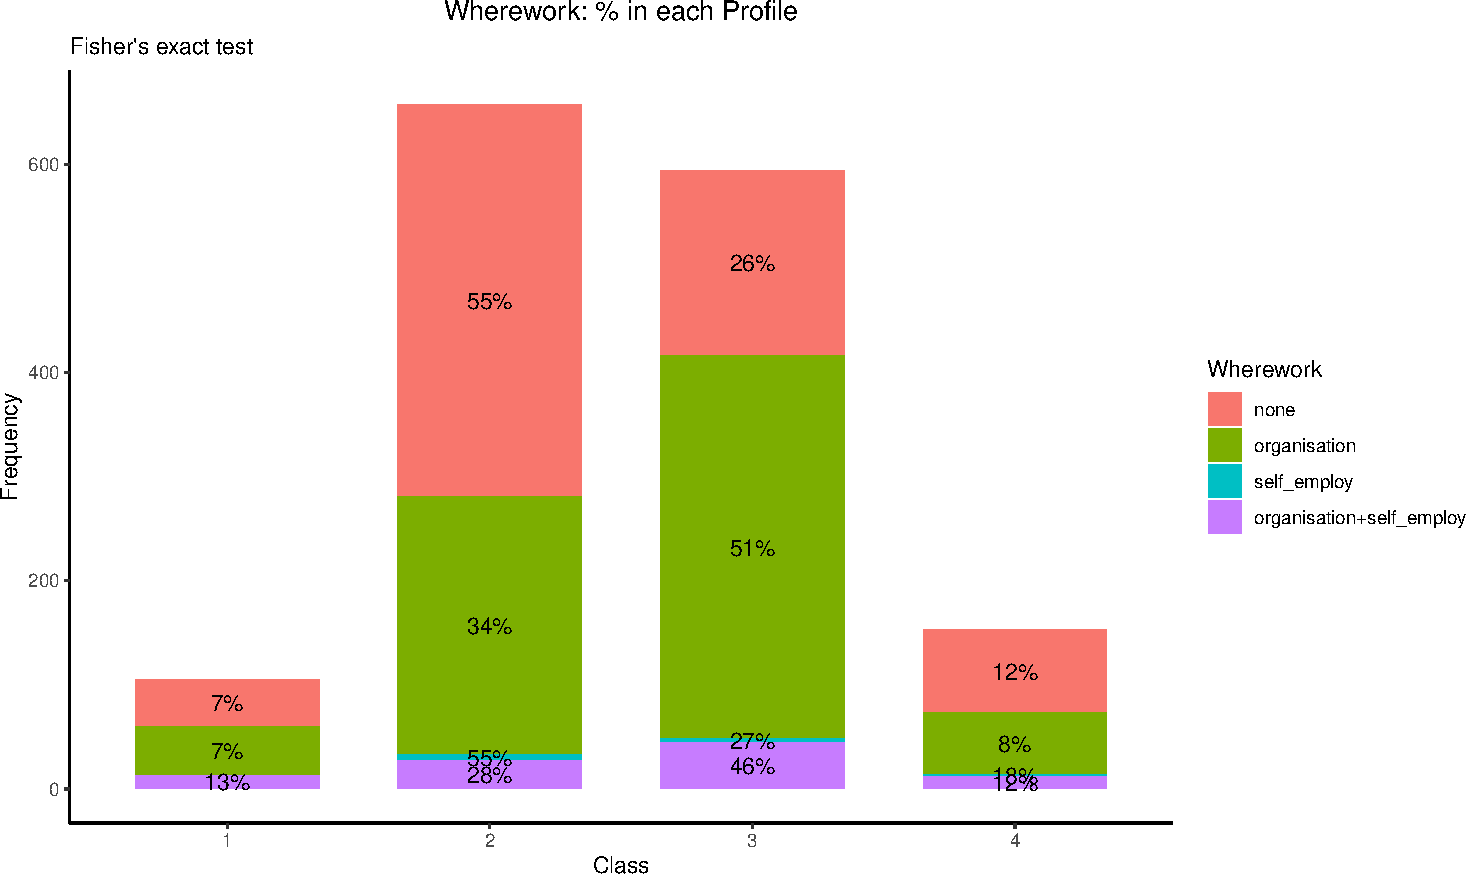
\includegraphics{lpa_analyses_files/figure-latex/unnamed-chunk-28-1} \end{center}

\newpage

\hypertarget{list-of-goodness-of-fit-indices}{%
\section{List of goodness of fit
indices}\label{list-of-goodness-of-fit-indices}}

A list and description of the GFI that can be computed for LPA models. -
LogLik: Log-likelihood of the data, given the model.

\begin{itemize}
\item
  AIC: Aikake information criterion; based on -2 log-likelihood, and
  penalized by number of parameters.\\
\item
  BIC: Bayesian information criterion; based on -2 log-likelihood, and
  penalized by number of parameters adjusted by sample size.\\
\item
  Entropy: A measure of classification uncertainty, reverse-coded so
  that 1 reflects complete certainty of classification, and 0 complete
  uncertainty (see Celeux \& Soromenho, 1996).\\
\item
  BLRT: bootstrapped likelihood test.\\
\item
  BLRT p-value: p-value for the bootstrapped likelihood ratio test.
\item
  AWE: Approximate weight of evidence; combines information on model fit
  and on classification errors (Celeux et al., 1997).\\
\item
  CAIC: Consistent Aikake information criterion; based on -2
  log-likelihood, and penalized by number of parameters adjusted by
  sample size.\\
\item
  CLC: Classification Likelihood Criterion; based on -2 log-likelihood,
  and penalized by the entropy (Biernacki, 1997).\\
\item
  KIC: Kullback information criterion; based on -2 log-likelihood, and
  penalized by 3 times the number of parameters -1 (Cavanaugh, 1999).\\
\item
  SABIC: Sample size-adjusted Bayesian information criterion (Sclove,
  1987).\\
\item
  ICL: Integrated completed likelihood (Biernacki, Celeux, \& Govaert,
  2000).\\
\item
  Prob. Min.: Minimum of the diagonal of the average latent class
  probabilities for most likely class membership, by assigned class. The
  minimum should be as high as possible, reflecting greater
  classification certainty (cases are assigned to classes they have a
  high probability of belonging to; see Jung \& Wickrama, 2008).\\
\item
  Prob. Max.: Maximum of the diagonal of the average latent class
  probabilities for most likely class membership, by assigned class. The
  maximum should also be as high as possible, reflecting greater
  classification certainty (cases are assigned to classes they have a
  high probability of belonging to).
\item
  N Min.: Proportion of the sample assigned to the smallest class (based
  on most likely class membership).\\
\item
  N Max.: Proportion of the sample assigned to the largest class (based
  on most likely class membership).
\end{itemize}

\end{document}
